\documentclass{article}
\usepackage[italian]{babel}

\usepackage[a4paper,top=2cm,bottom=2.4cm,left=2.4cm,right=3cm,marginparwidth=1.75cm]{geometry}

% Useful packages
\usepackage{graphicx}
\graphicspath{ {images/} }
\usepackage[colorlinks=true, allcolors=blue]{hyperref}
\usepackage{bold-extra}

\usepackage{enumitem}
\setlist[enumerate,1]{label=\arabic*{.}}
\setlist[enumerate,2]{label=\arabic{enumi}{.}\arabic*{.}}
\setlist[enumerate,3]{label=\arabic{enumi}{.}\arabic{enumii}{.}\arabic*{.}}
\setlist[enumerate,4]{label=\arabic{enumi}{.}\arabic{enumii}{.}\arabic{enumiii}{.}\arabic*{.}}



\title{Descrizione casi d'uso}
\author{Valerio Morelli}

\begin{document}


\section{Diagrammi dei casi d'uso}

\indent \indent Seguono ora i diagrammi dei casi d'uso e per ciasucuno di essi una dettagliata descrizione dei casi d'uso presenti. Per rendere il più possibile comoda la lettura da parte del lettore, gli autori hanno scelto di ordinare la descrizione dei casi d'uso secondo il loro identificativo numerico crescente. Tale identificativo è stato riportato anche sulle rappresentazioni grafiche dei diagrammi. 

\medskip

Si tenga inoltre presente che, al fine di non appesantire le rappresentazioni grafiche, sono state omesse le relazioni di associazione tra attore e caso d'uso qualora esse fossero state già esplicitate in altri diagrammi e ripeterle nell'attuale non avrebbe contribuito in modo indispensabile alla comprensione della logica del sistema. Sempre nel perseguimento di tale scopo si è scelto di colorare in grigio i casi d'uso presenti in un diagramma, ma originari di un'altro diagramma.

\medskip

 Il diagramma dei casi d'uso è composto da 5 \emph{packages} oltre al \emph{package} degli attori; nel dettaglio essi sono:

\medskip
\begin{itemize}[itemsep=0pt]
  \item \texttt{Gestione Cliente} (CU 01) - (CU 10)
  \item \texttt{Gestione Segreteria} (CU 11) - (CU 15)
  \item \texttt{Gestione Amministrazione} (CU 16) - (CU 23)
  \item \texttt{Gestione Sistema} (CU 24) - (CU 27)
  \item \texttt{Gestione Statistiche} (CU 28) - (CU 35)
\end{itemize}

\begin{figure}[h]
    \centering
    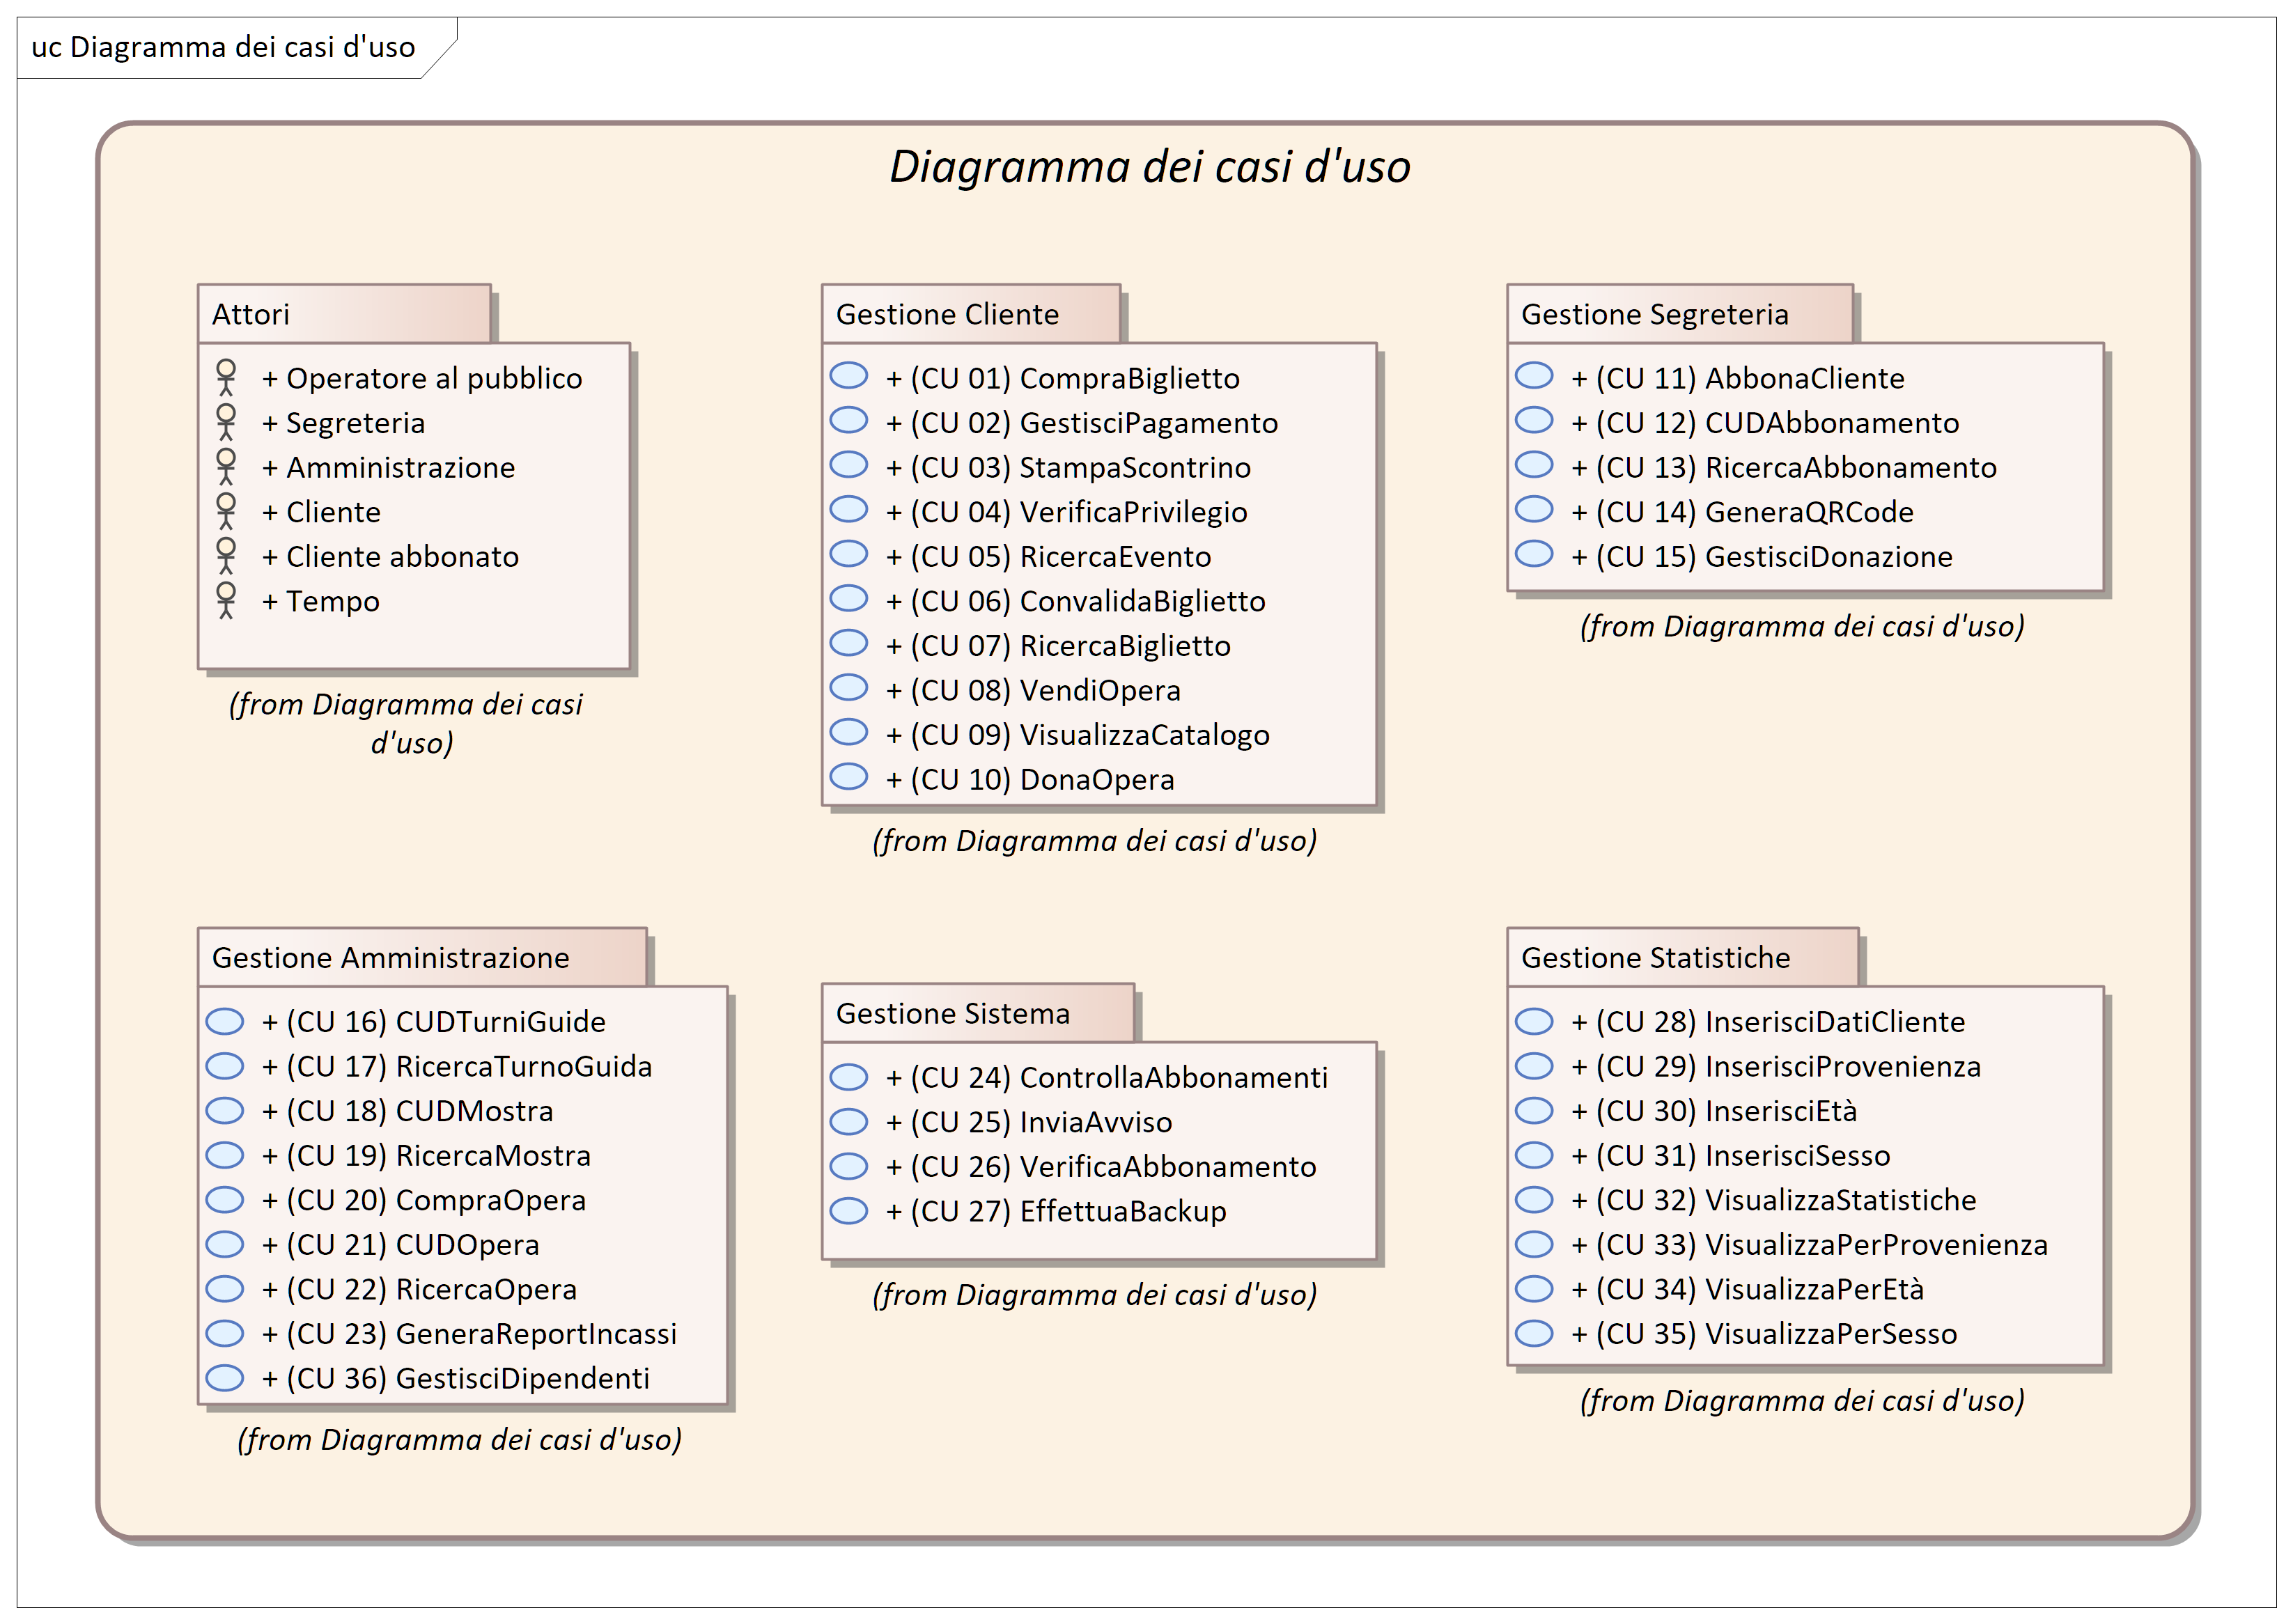
\includegraphics[width=1\textwidth]{Diagramma dei casi d'uso}
    \caption{diagramma dei casi d'uso: \textbf{Diagramma dei casi d'uso}}
    \label{fig:Diagramma dei casi d'uso}
\end{figure}



\newpage

\section{Gestione Cliente}

\indent\indent Il package degli attori contiene i 'soggetti' del dominio del problema in esame, ovvero coloro che interagiranno con il presente sistema al fine di svolgere il loro lavoro. Nel dettaglio i 6 attori sono:

\medskip
\begin{itemize}[itemsep=0pt]
  \item \texttt{Cliente}
  \item \texttt{Cliente abbonato}
  \item \texttt{Operatore al pubblico}
  \item \texttt{Segreteria}
  \item \texttt{Amministrazione}
  \item \texttt{Tempo}
\end{itemize}

\medskip
Si noti la relazione di generalizzazione che prende posto tra l'attore \emph{Cliente} e l'attore \emph{Cliente abbonato}. Mentre del secondo il sistema possiede le informazioni anagrafiche lasciate al momento della sua registrazione, non possiede che dati in forma anonima del \emph{Cliente}, ovvero di colui che usufruisce dei servizi offerti dal museo senza essere in possesso di un abbonamento. In altre parole, poiché il presente sistema non obbliga il \emph{Cliente} a registrarsi per accedere alla struttura e usufruire dei suoi servizi, gli unici dati che il sistema memorizza su di lui sono quelli (facoltativi) rilasciati in forma anonima per le statistiche.

\begin{figure}[h]
    \centering
    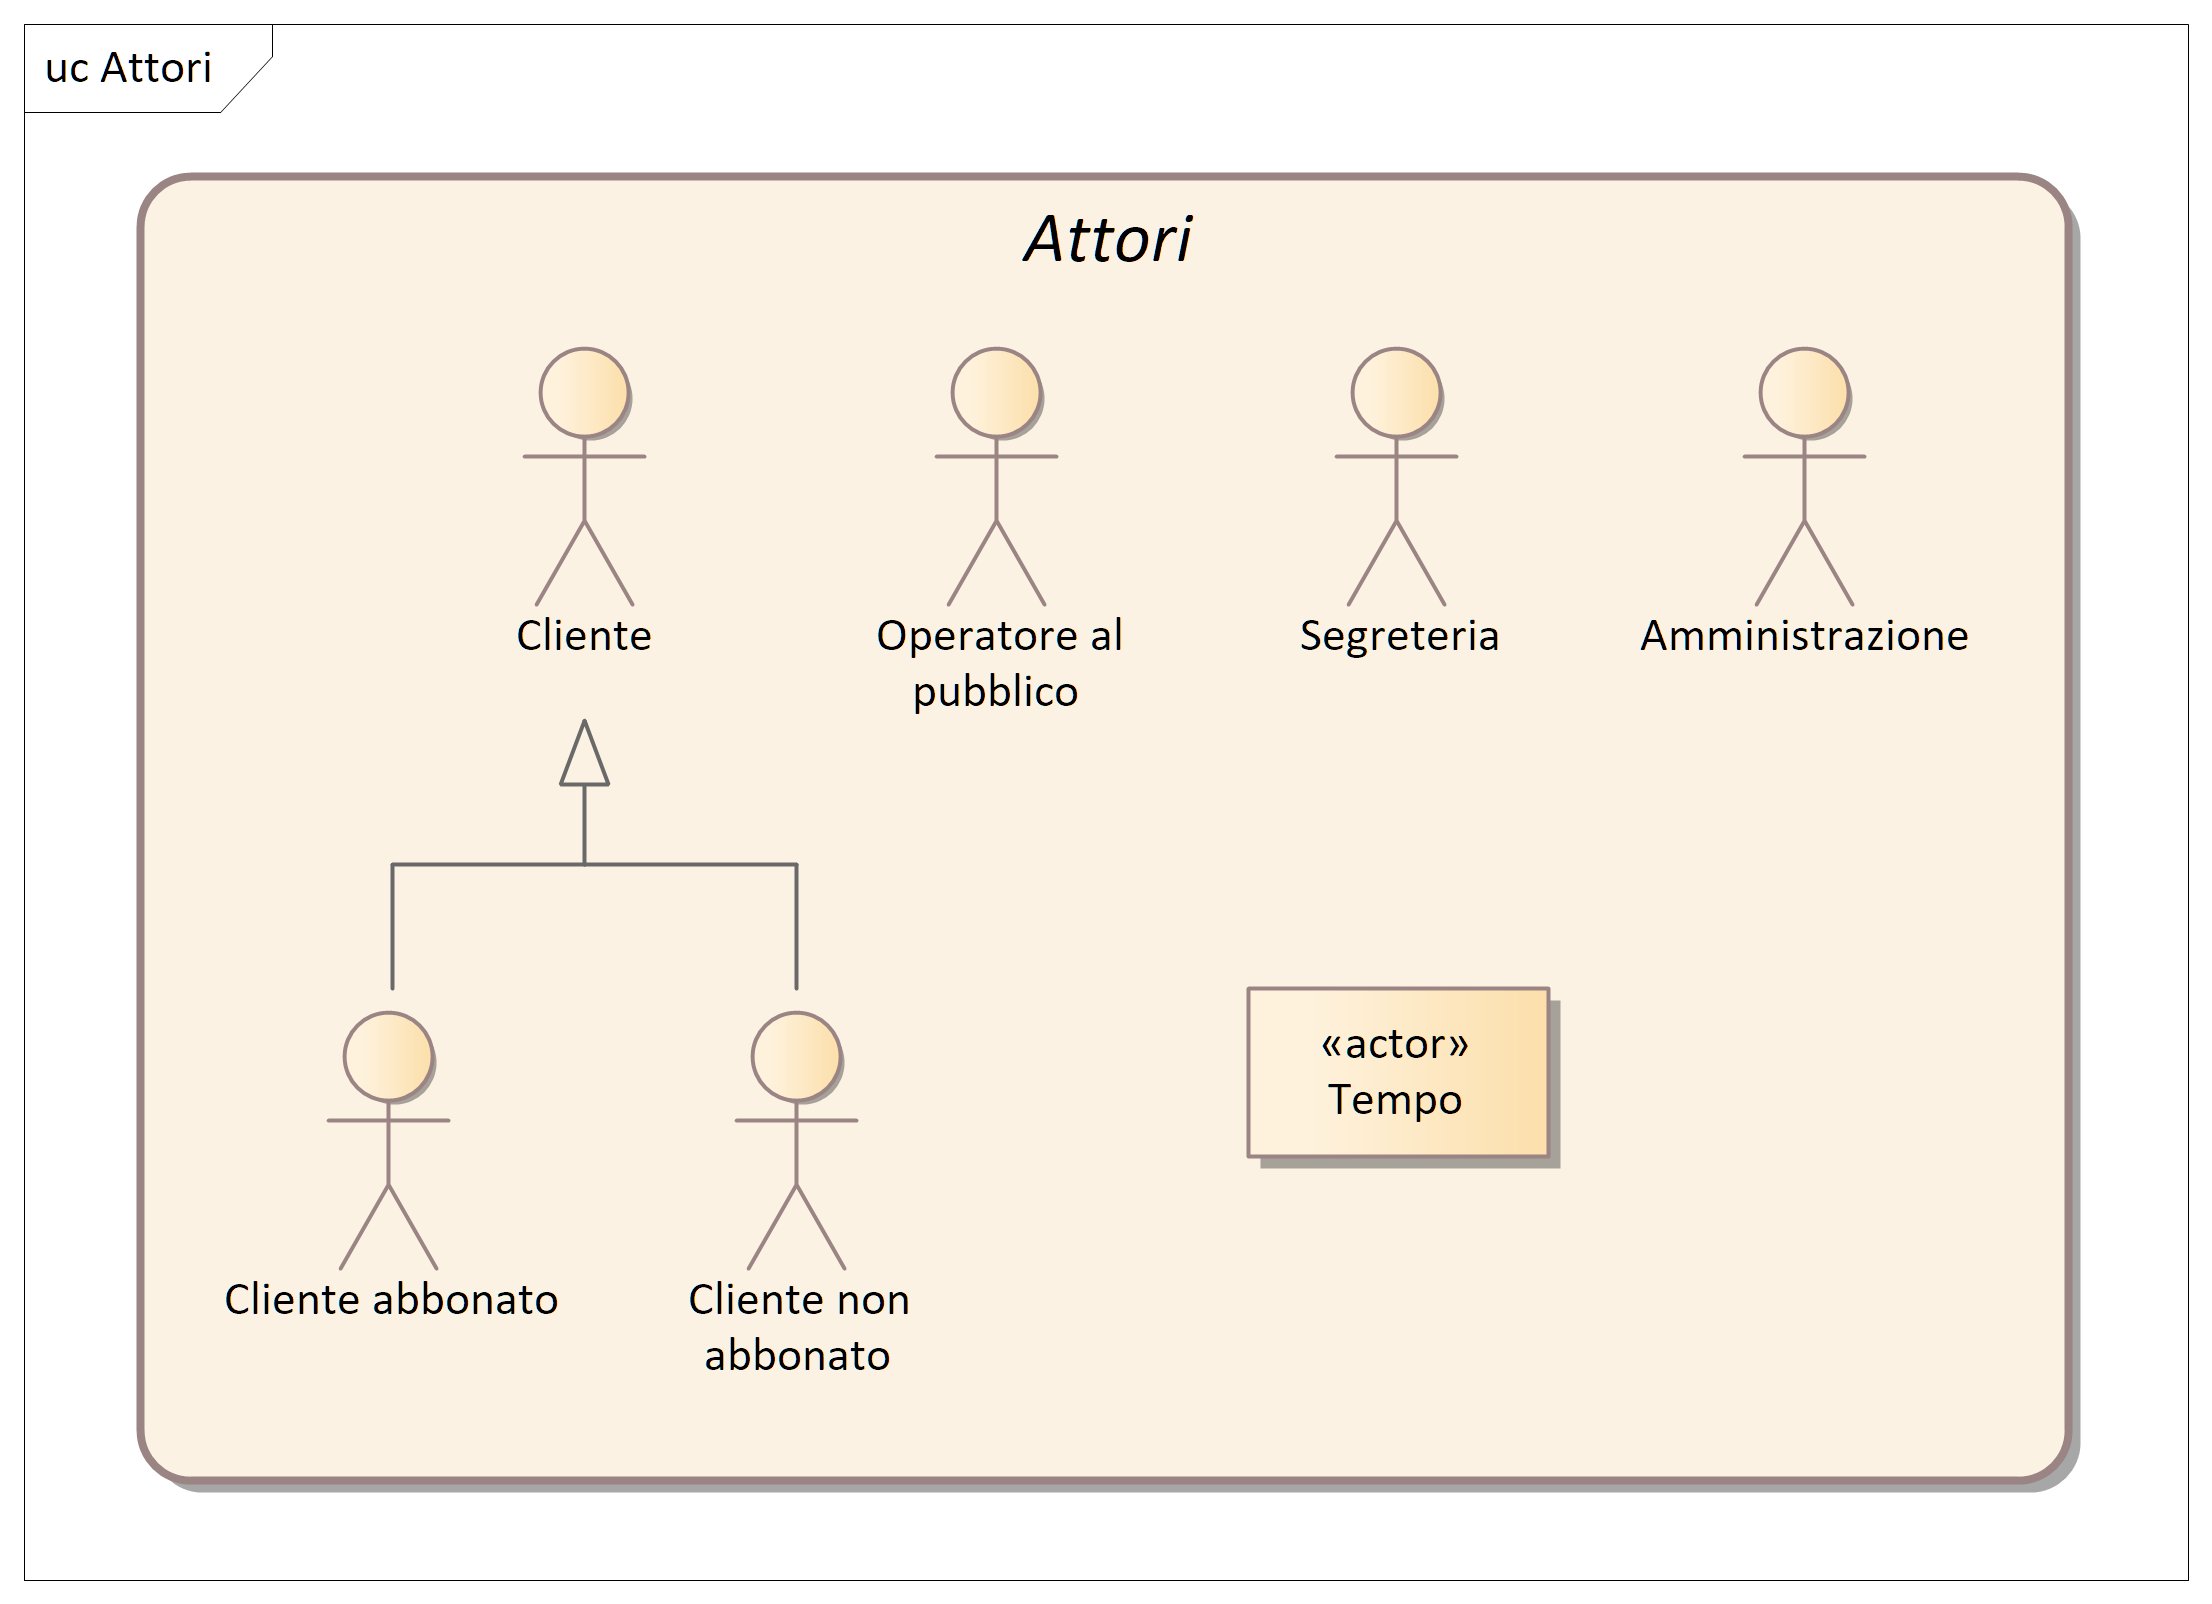
\includegraphics[width=1\textwidth]{Attori}
    \caption{Package: \textbf{Attori}}
    \label{fig:Attori}
\end{figure}












\newpage

\section{Gestione Cliente}

\indent\indent Il diagramma dei casi d'uso \textbf{Gestione Cliente} racchiude i casi d'uso volti a fornire servizi al cliente. Nel dettaglio, i casi d'uso di pertinenza sono:

\medskip
\begin{itemize}[itemsep=0pt]
  \item \texttt{CompraBiglietto} (CU 01)
  \item \texttt{GestisciPagamento} (CU 02)
  \item \texttt{StampaScontrino} (CU 03)
  \item \texttt{VerificaPrivilegio} (CU 04)
  \item \texttt{RicercaEvento} (CU 05)
  \item \texttt{ConvalidaBiglietto} (CU 06)
  \item \texttt{RicercaBiglietto} (CU 07)
  \item \texttt{VendiOpera} (CU 08)
  \item \texttt{VisualizzaCatalogo} (CU 09)
  \item \texttt{DonaOpera} (CU 10)
\end{itemize}

\medskip
Gli attori coinvolti in questi casi d'uso sono il \emph{Cliente abbonato}, generalizzato nell'attore \emph{Cliente}, e l'attore \emph{Operatore al pubblico}.

\medskip
Si noti che, poiché questo sistema informatico non prevede terminali sui quali il cliente può interfacciarsi direttamente, i casi d'uso istanziabili dal cliente hanno come attore secondario l'operatore al pubblico, il quale, una volta compresa la necessità del cliente, avvia la procedura interfacciandosi con il sistema.

\begin{figure}[h]
    \centering
    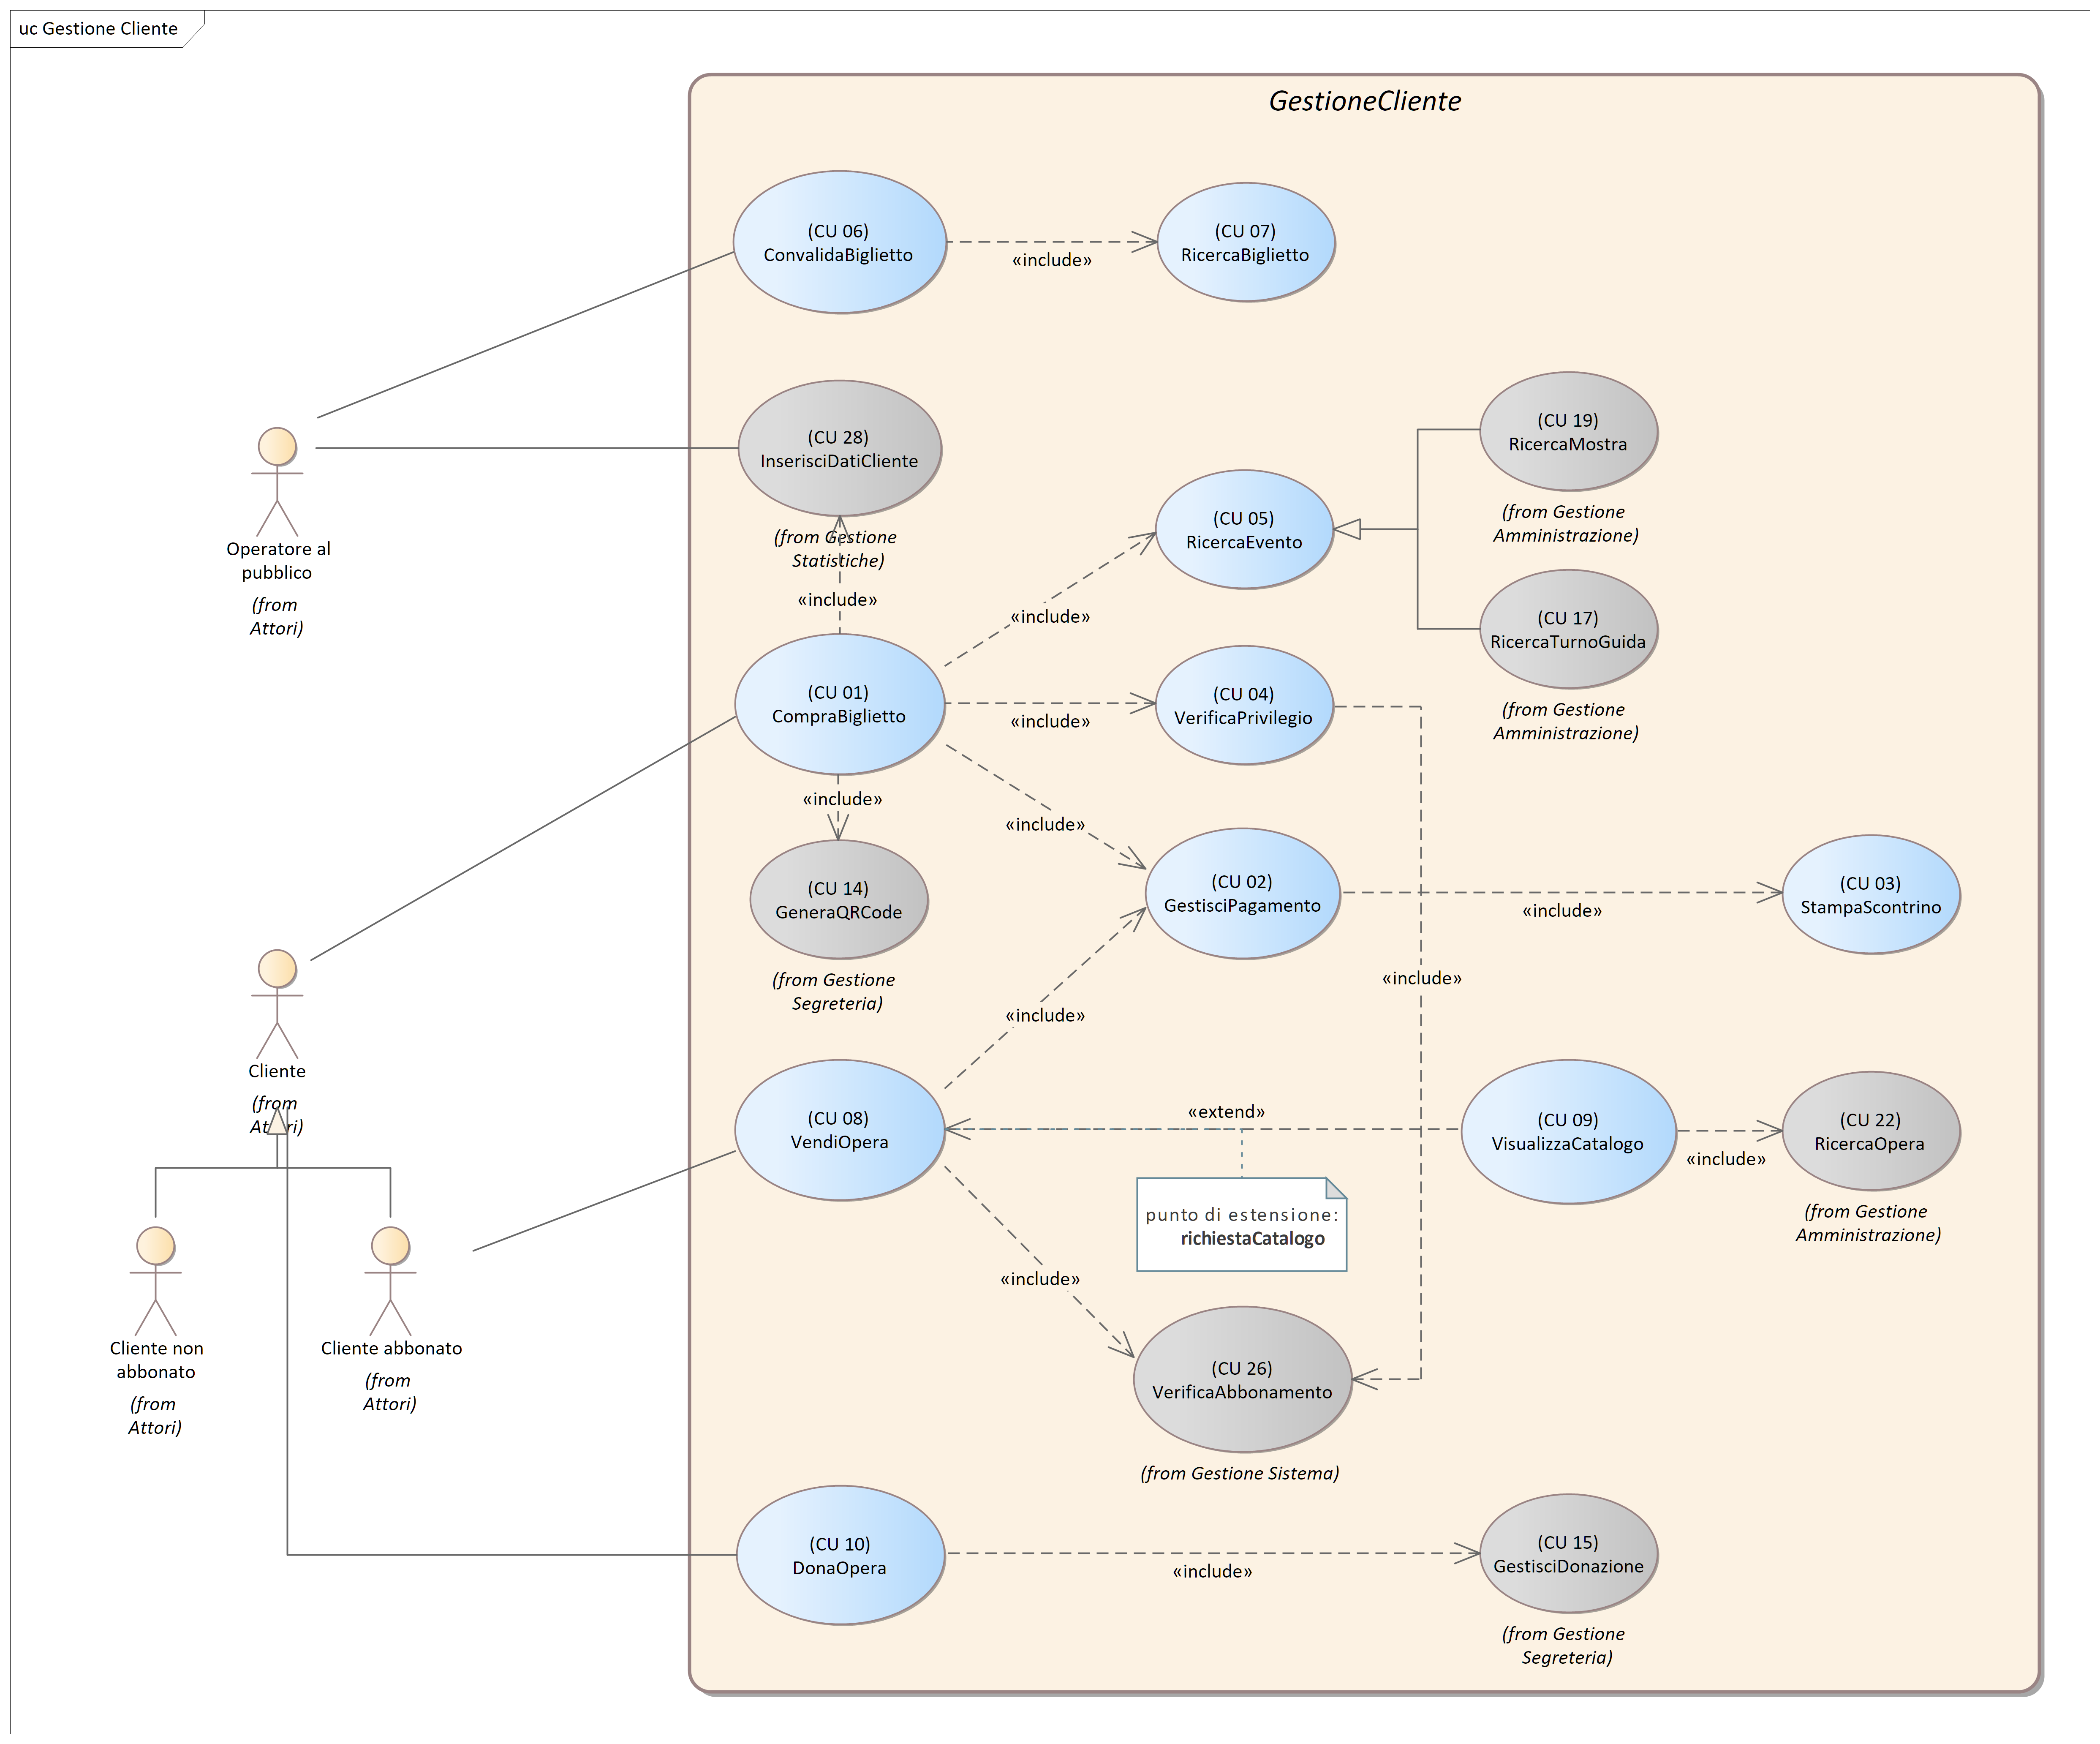
\includegraphics[width=0.92\textwidth]{Gestione Cliente}
    \caption{diagramma dei casi d'uso: \textbf{Gestione Cliente}}
    \label{fig:GestioneCliente}
\end{figure}

	

	\section*{CompraBiglietto (CU 01)}
	
	\indent\indent Questo caso d'uso consente l'acquisto di un biglietto per l'accesso al museo o ad una mostra.
	
	\paragraph{Attori primari:}Cliente.
	
	\paragraph{Attori secondari:}Operatore al pubblico.
	
	\paragraph{Precondizioni:}Nessuna.
	
	\paragraph{Postcondizioni:}Nessuna.
	
	\paragraph{Sequenza eventi principale:}

		\begin{enumerate}[itemsep=5pt,parsep=0pt]

		\item Il caso d'uso inizia quando l'attore primario esprime la volontà di acquistare un biglietto.

		\item L'attore secondario prende coscienza della volontà dell'attore primario e lo assiste nell'operazione.

		\item L'attore secondario effettua l'accesso con le sue credenziali se richiesto.

		\item \texttt{\textbf{if}} l'attore primario vuole accedere alla mostra:
			\begin{enumerate}	[leftmargin=28pt]
				\item L'attore secondario seleziona la mostra attuale.
				%\item \texttt{{include(RicercaMostra)}}.
  			\end{enumerate}	

		\item L'attore secondario inserisce nel sistema i dati relativi alla tipologia del biglietto.

		\item \texttt{\textbf{if}} l'attore primario richiede anche il servizio guida:
			\begin{enumerate}[leftmargin=28pt]
				\item  \texttt{{include(RicercaTurnoGuida)}}.
				\item L'attore secondario comunica all'attore primario gli orari dei turni delle guide disponibili.
				\item \texttt{\textbf{if}} c'è almeno un turno disponibile \texttt{\textbf{and}} l'attore primario ne sceglie uno:
					\begin{enumerate}[leftmargin=34pt]
						\item L'attore secondario inserisce la scelta dell'attore primario nel sistema.
					\end{enumerate}
  			\end{enumerate}	

		\item \texttt{\textbf{if}} l'attore primario comunica all'attore secondario di voler usufruire della tariffa ridotta:
			\begin{enumerate}[leftmargin=34pt]
				\item  \texttt{{include(VerificaPrivilegio)}}.
			\end{enumerate}

		\item Il sistema memorizza le informazioni e calcola il costo totale del biglietto, mostrando in un opportuno il resoconto dell'operazione.

		\item  \texttt{{include(InserisciDatiCliente)}}.

		\item  \texttt{{include(GestisciPagamento)}}.

		\item Il sistema genera un identificativo univoco per il biglietto.

		\item  \texttt{{include(GeneraQRCode)}}.

		\item Il sistema applica il codice QR sul fronte del biglietto e lo stampa.
	\end{enumerate}
	
	\paragraph{Sequenza eventi alternativa: \emph{PrivilegioNonVerificato}}
		\begin{enumerate}[itemsep=8pt,parsep=0pt]
				\item La sequenza di eventi alternativa inizia dopo il passo 6.1. della sequenza di eventi principale.
				\item Il sistema mostra un opportuno messaggio di errore comunicando all'attore secondario la non validità del privilegio necessario per poter usufruire della tariffa ridotta.
		\end{enumerate}

	\paragraph{Sequenza eventi alternativa: \emph{AbbonamentoScaduto}}
		\begin{enumerate}[itemsep=8pt,parsep=0pt]
				\item La sequenza di eventi alternativa inizia dopo il passo 6.1. della sequenza di eventi principale.
				\item Il sistema mostra un opportuno messaggio di errore comunicando all'attore secondario la non validità dell'abbonamento inserito.
		\end{enumerate}

	\paragraph{Sequenza eventi alternativa: \emph{PagamentoRifiutato}}
		\begin{enumerate}[itemsep=8pt,parsep=0pt]
				\item La sequenza di eventi alternativa inizia dopo il passo 8. della sequenza di eventi principale.
				\item Il sistema mostra un opportuno messaggio di errore comunicando all'attore primario l'errore avvenuto durante il pagamento ed esortandolo a riprovare.
		\end{enumerate}











\section*{GestisciPagamento (CU 02)}

    \indent\indent Questo caso d'uso permette di gestire il pagamento di un servizio offerto dal museo.
    
    \paragraph{Attori primari:}Segreteria, Operatore al pubblico.
	
	\paragraph{Attori secondari:}Cliente.
	
	\paragraph{Precondizioni:}
	\begin{enumerate}[itemsep=8pt,parsep=0pt]
		\item Il sistema sta elaborando la richiesta da parte del cliente di acquisto di un biglietto, di un abbonamento \texttt{\textbf{or}} di un'opera.
		\item L'attore primario ha comunicato al sistema il bene che il cliente deisdera acquistare.
	\end{enumerate}
	
	\paragraph{Postcondizioni:}
		\begin{enumerate}[itemsep=8pt,parsep=0pt]
			\item Il sistema ha registrato il pagamento.
		\end{enumerate}
	
	\paragraph{Sequenza eventi principale:}
\begin{enumerate}[itemsep=8pt,parsep=0pt]

    \item Il caso d'uso inizia quando l'attore primario deve gestire il pagamento di un acquisto effettuato da parte del cliente.

	\item Il sistema comunica all'attore primario il costo totale dell'acquisto.

	\item L'attore primario comunica all'attore secondario il totale da pagare e gli chiede la modalità di pagamento che desidera seguire.

	\item \texttt{\textbf{if}} l'attore secondario comunica di voler pagare in contanti:
		\begin{enumerate}[leftmargin=28pt]
			\item L'attore primario gestisce manualmente il pagamento usufruendo della cassa per erogare l'evenuale resto e riporre il denaro.
			\item L'attore primario comunica l'avvenuto pagamento al sistema.
		\end{enumerate}
	\item \texttt{\textbf{else if}} l'attore secondario comunica di voler pagare utilizzando il \emph{Point Of Sale}:
		\begin{enumerate}[leftmargin=28pt]
			\item L'attore primario consegna all'attore secondario il \emph{Point Of Sale}.
			\item L'attore secondario inserisce la sua carta di credito, di debito 	\texttt{\textbf{or}} prepagata, e segue i passaggi richiesti per autenticarla.
			%\item Il \emph{Point Of Sale} identifica la carta inserita e finalizza il pagamento mandando la richiesta di transazione al server della banca esercente della carta.
			\item Il sistema riceve l'esito della transazione dal \emph{Point Of Sale}.
		\end{enumerate}

		\item Il sistema registra l'avvenuto pagamento.
    \item \texttt{include(StampaScontrino)}
    
\end{enumerate}
    
	\paragraph{Sequenza eventi alternativa: \emph{TransazioneNonRiuscita}}
		\begin{enumerate}[itemsep=8pt,parsep=0pt]
				\item La sequenza di eventi alternativa inizia dopo il passo 5.3. della sequenza di eventi principale.
				\item Il sistema mostra un opportuno messaggio di errore comunicando all'attore primario l'errore avvenuto durante il pagamento ed esortandolo a ripetere l'operazione.
		\end{enumerate}



\newpage

\section*{StampaScontrino (CU 03)}

    \indent\indent Questo caso d'uso permette di stampare lo scontrino con l'importo pagato.
    
     
    \paragraph{Attori primari:}Segreteria, Operatore al pubblico.
	
	\paragraph{Attori secondari:}Cliente.
	
	\paragraph{Precondizioni:}
		\begin{enumerate}[itemsep=8pt,parsep=0pt]
			\item Il processo di pagamento terminato ed è andato a buon fine.
		\end{enumerate}
	
	\paragraph{Postcondizioni:} Nessuna.
	
	\paragraph{Sequenza eventi principale:}
\begin{enumerate}[itemsep=8pt,parsep=0pt]

    \item Il caso d'uso inizia quando l'attore primario deve stampare lo scontrino per l'avvenuto pagamento.

    \item Il sistema comunica al registratore di cassa telematico le informazioni del pagamento.

	\item L'attore primario attende l'avvenuta stampa e consegna all'attore secondario.
    

\end{enumerate}

	\paragraph{Sequenza eventi alternativa: \emph{ConnessioneAssente}}
		\begin{enumerate}[itemsep=8pt,parsep=0pt]
				\item La sequenza di eventi alternativa inizia dopo il passo 2. della sequenza di eventi principale.
				\item Il sistema mostra un opportuno messaggio di errore comunicando all'attore primario l'impossibilità di connessione da parte del registratore di cassa telematico, e lo esorta a ripovare \texttt{\textbf{or}} a riportare a mano lo scontrino su carta.
		\end{enumerate}




	
\newpage
    
\section*{VerificaPrivilegio (CU 04)}

    \indent\indent Questo caso d'uso permette di verificare il privilegio di un cliente ad aderire al costo ridotto o di essere esente dal pagamento per l'acquisto di un biglietto.
    
    \paragraph{Attori primari:}Operatore al pubblico.
	
	\paragraph{Attori secondari:}Cliente.
	
	\paragraph{Precondizioni:} 
		\begin{enumerate}[itemsep=8pt,parsep=0pt]
			\item Si è verificata la volonta da parte del cliente di acquistare un biglietto.
		\end{enumerate}

	
	\paragraph{Postcondizioni:}Nessuna.
	
	\paragraph{Sequenza eventi principale:}
\begin{enumerate}[itemsep=8pt,parsep=0pt]

    \item Il caso d'uso inizia quando l'attore primario desidera verificare se il cliente può usufruire dei privilegi di costo ridotto o nullo.

	\item L'attore primario chiede l'attore secondario quale privilegio desidera sfruttare.
    
    \item   \texttt{\textbf{if}} l'attore secondario chiede di utilizzare il privilegio sull'età :
        \begin{enumerate}[itemsep=8pt,parsep=0pt]
		\item L'attore primario chiede all'attore secondario di mostrare un documento d'identità.
			\item   \texttt{\textbf{if}} L'età dell'attore secondario è maggiore di 5 anni \texttt{\textbf{and}} minore di 18 anni \texttt{\textbf{or}} è maggiore di 60 anni : 
			        \begin{enumerate}[itemsep=8pt,parsep=0pt]
						\item L'attore primario conferma l'aderenza alla tariffa ridotta.
					\end{enumerate}

			\item   \texttt{\textbf{else if}} L'età dell'attore secondario è minore o aguale a 5 anni:
			        \begin{enumerate}[itemsep=8pt,parsep=0pt]
						\item L'attore primario conferma l'esenza dal pagamento.
					\end{enumerate}
        \end{enumerate}

    \item   \texttt{\textbf{else if}} l'attore secondario chiede di utilizzare il privilegio sull'occupazione :
        \begin{enumerate}[itemsep=8pt,parsep=0pt]
		\item L'attore primario chiede all'attore secondario di mostrare il badge di studente \texttt{\textbf{or}} il badge di professore.
			\item   \texttt{\textbf{if}} l'attore secondario ha consegnato il badge di studente \texttt{\textbf{and}} l'attore secondario ritiene valido il badge consegnatogli:
			        \begin{enumerate}[itemsep=8pt,parsep=0pt]
						\item L'attore primario conferma l'aderenza alla tariffa ridotta.
					\end{enumerate}

			\item   \texttt{\textbf{else if}} l'attore secondario ha consegnato il badge di professore \texttt{\textbf{and}} l'attore secondario ritiene valido il badge consegnatogli:
			        \begin{enumerate}[itemsep=8pt,parsep=0pt]
						\item L'attore primario conferma l'esenza dal pagamento.
					\end{enumerate}
        \end{enumerate}

    \item   \texttt{\textbf{else if}} l'attore secondario chiede di utilizzare il privilegio sul possedimento di certificato di invalidità:
        \begin{enumerate}[itemsep=8pt,parsep=0pt]
		\item L'attore primario chiede all'attore secondario di mostrare il certificato di invalidità.
		\item L'attore primario inserisce nel sistema il codice del certificato di invalidità.
			\item   \texttt{\textbf{if}} il sistema conferma la validità del certificato:
			        \begin{enumerate}[itemsep=8pt,parsep=0pt]
						\item L'attore primario conferma l'esenza dal pagamento.
					\end{enumerate}
        \end{enumerate}

    \item   \texttt{\textbf{else if}} l'attore secondario chiede di utilizzare il privilegio sul possedimento di abbonamento:
        \begin{enumerate}[itemsep=8pt,parsep=0pt]
		\item L'attore primario chiede all'attore secondario di mostrare il suo abbonamento.
	     \item   \texttt{include(VerificaAbbonamento)}
			\item   \texttt{\textbf{if}} l'abbonamento non è scaduto:
			        \begin{enumerate}[itemsep=8pt,parsep=0pt]
						\item L'attore primario conferma l'esenza dal pagamento.
					\end{enumerate}
        \end{enumerate}
        
        \item   \texttt{\textbf{else}} l'attore primario non applica alcuna riduzione al costo del biglietto.
        
\end{enumerate}

    \paragraph{Sequenza eventi alternativa:} Nessuna.    
    



\newpage

		\section*{RicercaEvento (CU 05)}
	
	\indent\indent Questo caso d'uso consente di ricercare un evento. 
	
	\paragraph{Attori primari:}Operatore al pubblico.
	
	\paragraph{Attori secondari:}Nessuno.
	
	\paragraph{Precondizioni:}Nessuna.
	
	\paragraph{Postcondizioni:}Nessuna.
	
	\paragraph{Sequenza eventi principale:}

		\begin{enumerate}[itemsep=8pt,parsep=0pt]

		\item Il caso d'uso inizia quando l'attore primario vuole effettuare la ricerca di un evento \texttt{\textbf{or}} il sistema deve effettuare la ricerca di un evento.

		\item \texttt{\textbf{if}} il caso d'uso è stato avviato dall'attore:
			\begin{enumerate}	[leftmargin=28pt]
				\item Il sistema chiede i criteri di ricerca.
				\item L'attore inserisce i criteri di ricerca richiesti.
  			\end{enumerate}	

		\item Il sistema registra i parametri di ricerca.

		\item \texttt{\textbf{for each}} evento nel database:
			\begin{enumerate}	[leftmargin=28pt]
				\item Il sistema controlla se l'evento soddisfa i criteri di ricerca.
				\item \texttt{\textbf{if}} l'evento soddisfa il criterio:
					\begin{enumerate}	[leftmargin=28pt]
						\item Il sistema aggiunge l'evento alla lista dei risultati.
		  			\end{enumerate}	
  			\end{enumerate}	

		\item \texttt{\textbf{if}} la lista dei risultati contiene almeno un evento:
			\begin{enumerate}	[leftmargin=28pt]
				\item Il sistema mostra la lista dei risultati con tutte le loro informazioni.
  			\end{enumerate}	

		\item \texttt{\textbf{else}}:
			\begin{enumerate}	[leftmargin=28pt]
				\item Il sistema comunica all'attore che nessun evento soddisfa il criterio specificato.
  			\end{enumerate}	
		
\end{enumerate}	
	
	\paragraph{Sequenza eventi alternativa:}Nessuna.
















\newpage 

		\section*{ConvalidaBiglietto (CU 06)}
	
	\indent\indent Questo caso d'uso consente di verificare la validità di un biglietto mediante il suo identificativo stampato  sul fronte sotto forma di codice QR. 
	
	\paragraph{Attori primari:}Operatore al pubblico.
	
	\paragraph{Attori secondari:}Nessuno.
	
	\paragraph{Precondizioni:}
			\begin{enumerate}	[itemsep=8pt,parsep=0pt]
				\item Il sistema ha autenticato l'attore primario.
				\item L'attore primario dispone di un biglietto con codice QR.
  			\end{enumerate}	
	
	\paragraph{Postcondizioni:}Nessuna.
	
	\paragraph{Sequenza eventi principale:}

		\begin{enumerate}[itemsep=8pt,parsep=0pt]
		
				\item Il caso d'uso inizia quando l'attore primario vuole eseguire la convalida di un biglietto. 
		
				\item Il sistema chiede il codice identificativo del biglietto.

				\item \texttt{\textbf{while}} il codice identificativo non corrisponde ad alcun biglietto memorizzato nel sistema:
					\begin{enumerate}	[leftmargin=28pt]
						\item L'attore primario inserisce il codice identificativo eseguendo una scannerizzazione del codice QR stampato sul fronte del biglietto.
						\item \texttt{include(RicercaBiglietto)}
		  			\end{enumerate}	

				\item \texttt{\textbf{if}} la data attuale conicide con il giorno di validità del biglietto:
					\begin{enumerate}	[leftmargin=28pt]
						\item Il sistema mostra un opportuno messaggio di successo dell'operazione.
		  			\end{enumerate}	
				\item \texttt{\textbf{else}}:
					\begin{enumerate}	[leftmargin=28pt]
						\item Il sistema mostra un opportuno messaggio di errore.
		  			\end{enumerate}	
				
		\end{enumerate}	
	
	\paragraph{Sequenza eventi alternativa: \emph{IdentificativoNonTrovato}}

		\begin{enumerate}[itemsep=8pt,parsep=0pt]
				\item La sequenza di eventi alternativa inizia dopo il passo 3.2. della sequenza di eventi principale.
				\item Il sistema mostra un opportuno messaggio di errore comunicando all'attore l'inesistenza dell'identificativo all'interno del database ed esortandolo a ripetere il processo di scannerizzazione.
				\item La sequenza di eventi principale prosegue dal punto 3.
		\end{enumerate}





















\newpage 

		\section*{RicercaBiglietto (CU 07)}
	
	\indent\indent Questo caso d'uso consente di ricercare un biglietto nel database del sistema mediante il suo identificativo.
	
	\paragraph{Attori primari:}Operatore al pubblico.
	
	\paragraph{Attori secondari:}Nessuno.
	
	\paragraph{Precondizioni:}
			\begin{enumerate}	[itemsep=8pt,parsep=0pt]
				\item L'attore primario ha inserito il codice identificativo del biglietto nel sistema.
  			\end{enumerate}	
	
	\paragraph{Postcondizioni:}Nessuna.
	
	\paragraph{Sequenza eventi principale:}

		\begin{enumerate}[itemsep=8pt,parsep=0pt]
		
				\item Il caso d'uso inizia quando l'attore primario vuole effettuare la ricerca di un biglietto \texttt{\textbf{or}} il sistema deve effettuare la ricerca di un biglietto.
		
				\item Il sistema ottiene il codice identificativo del biglietto.

				\item \texttt{\textbf{for each}} biglietto nel database dei biglietti:
					\begin{enumerate}	[leftmargin=28pt]
						\item \texttt{\textbf{if}} l'identificativo del biglietto coincide con l'identificativo fornito al sistema:
							\begin{enumerate}	[leftmargin=28pt]
								\item Il sistema raccoglie tutte le informazioni del biglietto.
				  			\end{enumerate}
		  			\end{enumerate}	

				\item \texttt{\textbf{if}} la ricerca non ha prodotto alcun risultato:
					\begin{enumerate}	[leftmargin=28pt]
						\item Il sistema mostra un opportuno messaggio di errore.
		  			\end{enumerate}
				\item \texttt{\textbf{else if}} il caso d'uso è stato avviato dall'attore primario:
					\begin{enumerate}	[leftmargin=28pt]
						\item Il sistema mostra un opportuno messaggio di successo dell'operazione.
						\item Il sistema mostra, in una schermata opportuna, tutte le informazioni del biglietto, tra le quali la sua tipologia e l'eventuale presenza del servizio di guida.
					\end{enumerate}
				
		\end{enumerate}	
	
	\paragraph{Sequenza eventi alternativa:} Nessuna.

















\newpage 

		\section*{VendiOpera (CU 08)}
	
	\indent\indent Questo caso d'uso consente la vendita di un'opera da parte del museo.
	
	\paragraph{Attori primari:}Cliente abbonato.
	
	\paragraph{Attori secondari:}Operatore al pubblico.
	
	\paragraph{Precondizioni:}
			\begin{enumerate}	[itemsep=8pt,parsep=0pt]
				\item L'attore primario deve disporre di un abbonamento valido.
  			\end{enumerate}	
	
	\paragraph{Postcondizioni:}
			\begin{enumerate}	[itemsep=8pt,parsep=0pt]
				\item  Nel caso in cui l'operazione sia andata a buon fine, il sistema ha segnato come vendute le opere oggetto di transazione.
  			\end{enumerate}	
	
	\paragraph{Sequenza eventi principale:}

		\begin{enumerate}[itemsep=8pt,parsep=0pt]
		
				\item Il caso d'uso inizia quando l'attore primario esprime la volontà di acquistare un'opera di una mostra.
		
				\item L'attore secondario riceve la richiesta e chiede all'attore primario di mostrare il suo abbonamento.

				\item \texttt{include(VerificaAbbonamento)}

				\item \texttt{extention point: richiestaCatalogo}

				\item \texttt{\textbf{for each}} opera scelta dall'attore primario:
					\begin{enumerate}	[leftmargin=28pt]
						\item L'attore secondario aggiunge l'opera al carrello.
		  			\end{enumerate}
				\item L'attore secondario comunica al sistema la conferma dell'operazione.
				\item \texttt{include(GestisciPagamento)}
				\item \texttt{\textbf{for each}} opera venduta:
					\begin{enumerate}	[leftmargin=28pt]
						\item Il sistema segna come venduta l'opera.
		  			\end{enumerate}
  			\end{enumerate}				

	\paragraph{Sequenza eventi alternativa: \emph{OperazioneAnnullata}}
		\begin{enumerate}[itemsep=8pt,parsep=0pt]
				\item La sequenza di eventi alternativa inizia in qualunque momento.
				\item L'attore primario annulla l'acquisto delle opere.
		\end{enumerate}

	\paragraph{Sequenza eventi alternativa: \emph{AbbonamentoScaduto}}
		\begin{enumerate}[itemsep=8pt,parsep=0pt]
				\item La sequenza di eventi alternativa inizia dopo il passo 3. della sequenza di eventi principale.
				\item Il sistema mostra un opportuno messaggio di errore comunicando all'attore secondario la non validità dell'abbonamento inserito.
		\end{enumerate}

	\paragraph{Sequenza eventi alternativa: \emph{PagamentoRifiutato}}
		\begin{enumerate}[itemsep=8pt,parsep=0pt]
				\item La sequenza di eventi alternativa inizia dopo il passo 7. della sequenza di eventi principale.
				\item Il sistema mostra un opportuno messaggio di errore comunicando all'attore primario l'errore avvenuto durante il pagamento ed esortandolo a riprovare.
		\end{enumerate}













\newpage

\section*{VisualizzaCatalogo (CU 09)}

    \indent\indent Questo caso d'uso permette di generare ed eventualmente stampare una lista delle opere apparteneti alle mostre del museo ed in quanto tali vendibili al cliente richiedente.
    
    \paragraph{Attori primari:}Operatore al pubblico.
	
	\paragraph{Attori secondari:}Nessuno.
	
	\paragraph{Precondizioni del segmento 1:}
\begin{enumerate}[itemsep=8pt,parsep=0pt]
	\item L'attore secondario ha richiesto esplicitamente la volotà di visualizzare il catalogo delle opere vendibili.
\end{enumerate}
	
	\paragraph{Postcondizioni del segmento 1:}Nessuna.
	
	\paragraph{Sequenza eventi principale:}
\begin{enumerate}[itemsep=8pt,parsep=0pt]
    \item Il caso d'uso inizia quando l'attore primario riceve la richiesta di visualizzare il catalogo delle opere vendibili.
    
    \item \texttt{\textbf{for each}} mostra nel database delle mostre:
		\begin{enumerate}	[leftmargin=28pt]
		    \item   \texttt{include(RicercaMostra)}
			\item Il sistema genera una presentazione della mostra.
		    \item \texttt{\textbf{for each}} opera nella mostra:
				\begin{enumerate}	[leftmargin=28pt]
				    \item   \texttt{include(RicercaOpera)}
					\item Il sistema genera una presentazione dell'opera e la aggiunge alla presentazione della mostra.
			    \end{enumerate}
			\item Il sistema aggiunge la presentazione della mostra al catalogo.
		\end{enumerate}
	\item Il sistema mostra a schermo il catalogo generato, offrendo all'attore primario la possibilità di mandarlo in stampa.
    
\end{enumerate}
    
    
	\paragraph{Sequenza eventi alternativa del segmento 1: \emph{NessunaOperaVendibile}}
		\begin{enumerate}[itemsep=8pt,parsep=0pt]
				\item La sequenza di eventi alternativa inizia dopo il passo 3. della sequenza di eventi principale.
				\item Il sistema comunica all'attore primario l'assenza di opere vendibili e lo esorta a portare a termine l'operazione di vendita.
		\end{enumerate}
   










\newpage 

		\section*{DonaOpera (CU 10)}
	
	\indent\indent Questo caso d'uso consente la donazione di un'opera da parte di un cliente.
	
	\paragraph{Attori primari:}Cliente.
	
	\paragraph{Attori secondari:}Operatore al pubblico, Segreteria.
	
	\paragraph{Precondizioni:}Nessuna.
	
	\paragraph{Postcondizioni:}
		\begin{enumerate}[itemsep=8pt,parsep=0pt]
				\item Il sistema ha memorizzato la richiesta insieme a tutti i dati dell'opera in fase di donazione.
		\end{enumerate}	
	
	\paragraph{Sequenza eventi principale:}

		\begin{enumerate}[itemsep=8pt,parsep=0pt]
		
				\item Il caso d'uso inizia quando l'attore primario esprime la volontà di donare un'opera al museo.
		
				\item L'attore secondario \emph{Operatore al pubblico} riceve la richiesta ed inserisce nel sistema il nome, l'autore, le dimensioni, il tipo e l'immagine dell'opera.

				\item L'attore secondario \emph{Operatore al pubblico} chiede all'attore primario anche un indirizzo di posta elettronica attraverso il quale verrà comunicata la scelta della segreteria.

				\item L'attore secondario \emph{Operatore al pubblico} ripone l'opera in un magazzino appropriato in attesa dell'esito della richiesta.

				\item Il sistema registra le informazioni e notifica l'attore \emph{Segreteria} della richiesta.

				\item \texttt{include(GestisciDonazione)}						
		
		\end{enumerate}	

	\paragraph{Sequenza eventi alternativa:}Nessuna.






















































































































\newpage

\section{Gestione Segreteria}

\indent\indent Il diagramma dei casi d'uso \textbf{Gestione Segreteria} racchiude i casi d'uso necessari all'attore \emph{Segreteria} per svolgere le sue operazioni orientate a migliorare il lato servizio-cliente. Nel dettaglio, i casi d'uso di pertinenza sono:
\medskip
\begin{itemize}[itemsep=4pt]
  \item \texttt{AbbonaCliente} (CU 11)
  \item \texttt{CUDAbbonamento} (CU 12)
  \item \texttt{RicercaAbbonamento} (CU 13)
  \item \texttt{GeneraQRCode} (CU 14)
  \item \texttt{GestisciDonazione} (CU 15)
\end{itemize}
\medskip
L'attore coinvolto in questi casi d'uso è la \emph{Segreteria}.

\begin{figure}[h]
    \centering
    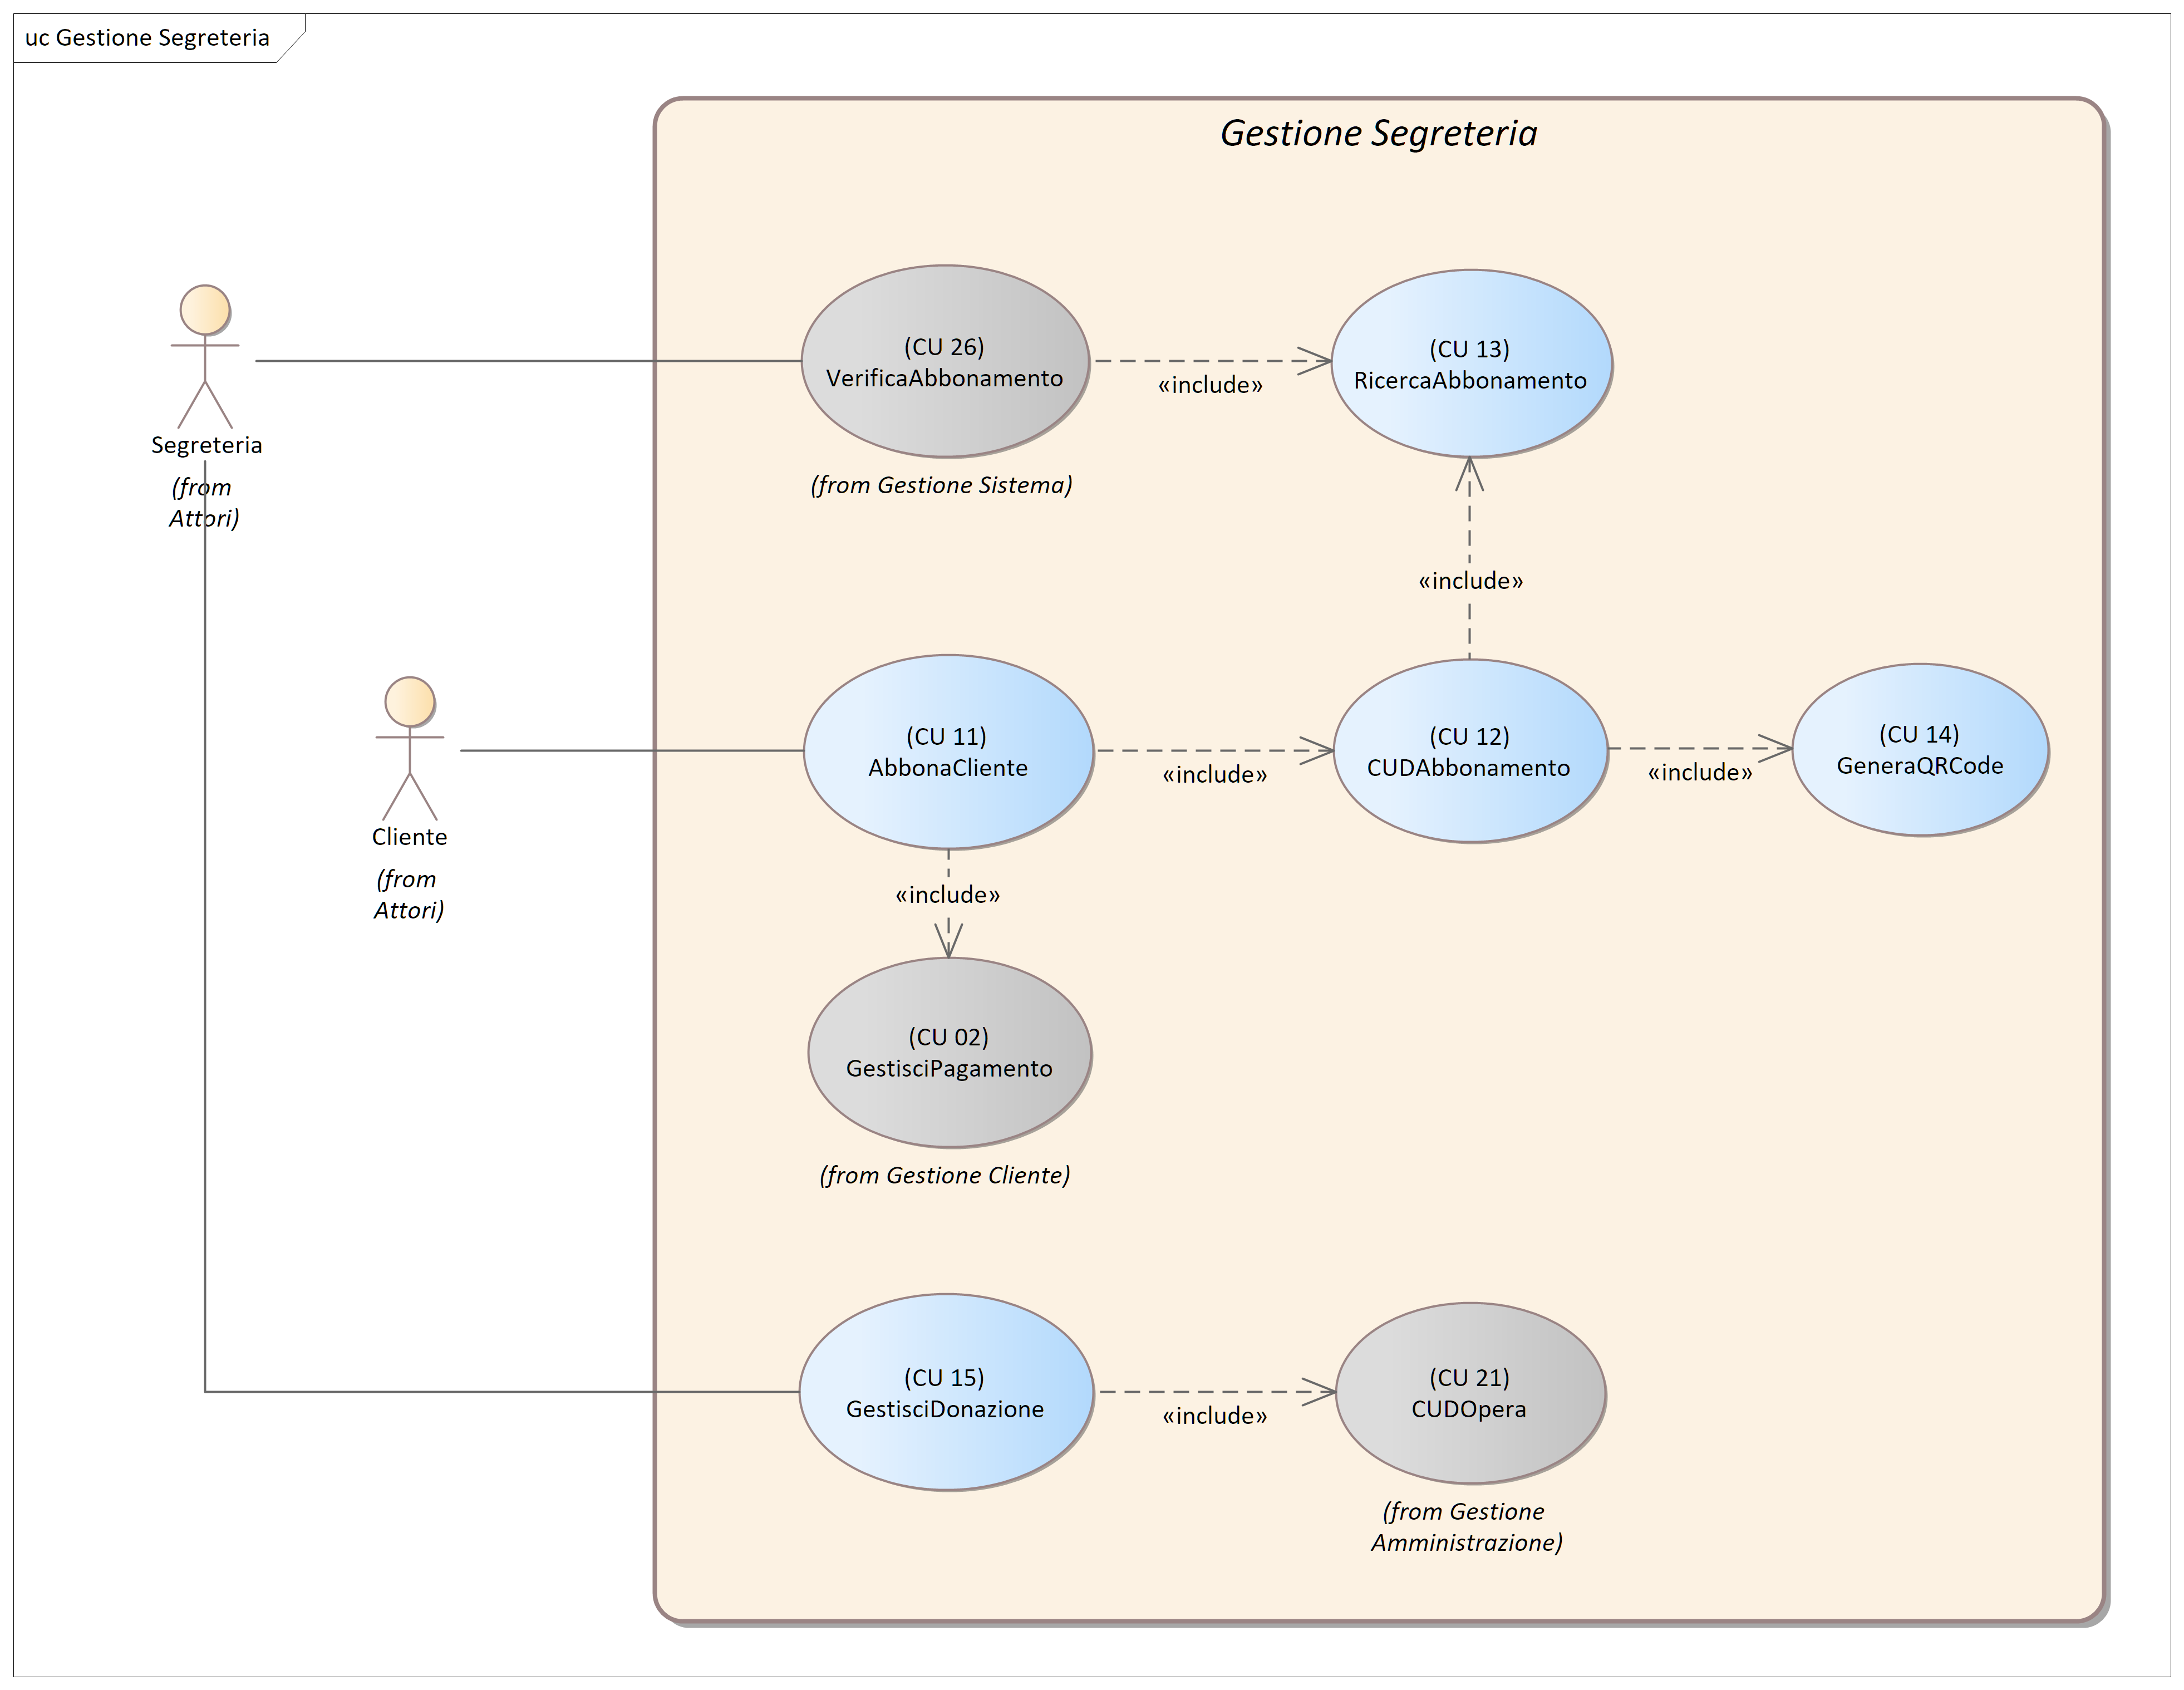
\includegraphics[width=1\textwidth]{Gestione Segreteria}
    \caption{diagramma dei casi d'uso: \textbf{Gestione Segreteria}}
    \label{fig:GestioneSegreteria}
\end{figure}





\newpage
\section*{AbbonaCliente (CU 11)}
	
	\indent\indent Questo caso d'uso consente la creazione di un abbonamento per un cliente non abbonato e il rinnovo di un abbonamento per un cliente abbonato.

	\paragraph{Attori primari:}Cliente non abbonato.

	\paragraph{Attori secondari:}Segreteria.

	\paragraph{Precondizioni:}Nessuno.

	\paragraph{Postcondizioni:}%(Il cliente ha pagato l'abbonamento?)(oppure qualcosa che riguarda la memorizzazione del nuovo abbonamento?)(o niente?).
	\begin{enumerate}[itemsep=8pt,parsep=0pt]
		\item Il sistema ha memorizzato il nuovo abbonamento nel database degli abbonamenti.
		\item Il sistema ha memorizzato il pagamento ricevuto.
	\end{enumerate}

	\paragraph{Sequenza eventi principale:}

	\begin{enumerate}[itemsep=8pt,parsep=0pt]

		\item Il caso d'uso inizia quando l'attore primario esprime la volontà di abbonarsi o di rinnovare il suo abbonamento.
		\item L'attore secondario prende coscienza della volontà dell'attore primario e lo assiste nell'operazione.
		\item \texttt{\textbf{if}} l'attore primario vuole abbonarsi:
			\begin{enumerate}	[leftmargin=28pt]
				\item L'attore secondario richiede all'attore primario i dati anagrafici e li registra nel sistema.
			\end{enumerate}
		\item \texttt{\textbf{else if}} l'attore primario vuole rinnovare il suo abbonamento:
			\begin{enumerate}	[leftmargin=28pt]
				\item L'attore secondario chiede all'attore primario di mostrare il suo abbonamento.
				\item L'attore secondario inserisce il codice identificativo eseguendo una scannerizzazione del codice QR stampato sul fronte dell'abbonamento.
				\item \texttt{include(RicercaAbbonamento)}
			\end{enumerate}
		\item L'attore secondario informa l'attore primario sulle tipologie di abbonamento disponibili in base alla loro durata e al loro costo, quindi chiede all'attore secondario i dati necessari per l'abbonamento.
		\item L'attore primario sceglie una tipologia di abbonamento e comunica all'attore secondario i dati richiesti. 
		\item L'attore secondario inserisce i dati nel sistema.
		\item  \texttt{include(CUDAbbonamento)}
		\item L'attore secondario comunica all'attore primario l'importo da pagare.
		\item  \texttt{include(GestisciPagamento)}
		%Qui ci sarebbe la necessità di mostrare sullo schermo l'operazione ben riuscita del pagamento, e dovrebbe venire eseguita in Gestisci pagamento, perciò qui non lo includo.
		\item L'attore secondario comunica all'attore primario l'esito positivo dell'operazione.
		\item Il sistema applica il codice QR sul fronte dell'abbonamento e lo stampa.
		
	\end{enumerate}
	
	\paragraph{Sequenza eventi alternativa:} \textbf{\textit{OperazioneAnnullata}}.
	\begin{enumerate}[itemsep=8pt,parsep=0pt]
	\item La sequenza di eventi alternativa inizia in qualunque momento.
	\item L'attore primario annulla la richiesta di abbonarsi.
	\end{enumerate}
	
	%\paragraph{Sequenza eventi alternativa:} \textbf{\textit{CreazioneAbbonamentoNonRiuscita}}.
	%%\begin{enumerate}[itemsep=8pt,parsep=0pt]
	%\item La sequenza di eventi alternativa inizia dopo il passo 6. della sequenza di eventi principale.
	%\item Il sistema mostra un opportuno messaggio di errore comunicando all'attore secondario l'esito negativo dell'operazione.
	%\end{enumerate}
	
	\paragraph{Sequenza eventi alternativa:} \textbf{\textit{PagamentoRifiutato}}.
	\begin{enumerate}[itemsep=8pt,parsep=0pt]
	\item La sequenza di eventi alternativa inizia dopo il passo 9. della sequenza di eventi principale.
	\item Il sistema mostra un opportuno messaggio di errore comunicando all'attore primario l'errore avvenuto ed esortandolo a riprovare.
	\end{enumerate}
	



\newpage	
\section*{CUDAbbonamento (CU 12)}
	
	\indent\indent Questo caso d'uso consente di eseguire la creazione, la modifica o l'eliminazione di un abbonamento.
	
	\paragraph{Attori primari:}Segreteria.
	
	\paragraph{Attori secondari:}Nessuno.
	
	\paragraph{Precondizioni:}Nessuna.
	
	\paragraph{Postcondizioni:}
			\begin{enumerate}	[leftmargin=28pt]
\item Il sistema ha memorizzato le eventuali modifiche nel database degli abbonamenti.
\end{enumerate}
	
	\paragraph{Sequenza eventi principale:}

	\begin{enumerate}[itemsep=8pt,parsep=0pt]

		\item Il caso d'uso inizia quando l'attore primario vuole eseguire un'operazione CUD relativa all'abbonamento.

		\item \texttt{\textbf{if}} l'attore primario vuole creare un nuovo abbonamento:
			\begin{enumerate}	[leftmargin=28pt]
			    \item L'attore primario inserisce i dati nel sistema.
			 %   \item \texttt{include(RicercaAbbonamento)}
			%    \item \texttt{\textbf{if}} l'abbonamento è già presente:
		    	%\begin{enumerate}	[leftmargin=28pt]
			%	    \item  Il sistema mostra un messaggio di errore.
			%	\end{enumerate}
			%	\item \texttt{\textbf{else}}
		    	%\begin{enumerate}	[leftmargin=28pt]
				    \item  Il sistema provvede a memorizzare i dati.
					\item Il sistema genera un identificativo univoco per l'abbonamento.
				    \item \texttt{include(GeneraQRCode)}
                    	    \item Il sistema inserisce il codice QR nell'abbonamento.
				    \item Il sistema mostra a schermo l'abbonamento creato e un messaggio contenente l'esito dell'operazione.
			%	\end{enumerate}
  			\end{enumerate}	

		\item \texttt{\textbf{else if}}  l’attore vuole modificare l'abbonamento esistente:
			\begin{enumerate}[leftmargin=28pt]
			   \item  \texttt{{include(RicercaAbbonamento)}}
			   \item \texttt{\textbf{if}} l'abbonamento viene trovato:
			    \begin{enumerate}	[leftmargin=28pt]
			        \item l'attore primario aggiorna i dati dell'abbonamento trovato.
			        \item  Il sistema provvede a salvare le modifiche.
                \end{enumerate}
  			\end{enumerate}	
  			
  		\item \texttt{\textbf{else if}} l'attore primario  \texttt{\textbf{or}} il sistema vuole eliminare l'abbonamento:
		\begin{enumerate}	[leftmargin=28pt]
		\item \texttt{\textbf{if}} il caso d'uso è stato attivato dall'attore primario
        \begin{enumerate}	[leftmargin=28pt]
				\item L'attore secondario chiede al cliente di mostrare il suo abbonamento.
				\item L'attore secondario inserisce il codice identificativo eseguendo una scannerizzazione del codice QR stampato sul fronte dell'abbonamento.
	       	\item  \texttt{include(RicercaAbbonamento)}
		    \item  Il sistema mostra un messaggio di conferma.
	   		\item \texttt{\textbf{if}}  l'attore primario conferma l'operazione:
	    	\begin{enumerate}	[leftmargin=28pt]
	    	    \item  Il sistema provvede ad eliminare l'abbonamento.
		    \end{enumerate}
		\end{enumerate}
	    \item \texttt{\textbf{else if}} il caso d'uso è stato attivato dal sistema:
        \begin{enumerate}	[leftmargin=28pt]
        	\item  \texttt{include(RicercaAbbonamento)}
	    	 \item  Il sistema provvede ad eliminare l'abbonamento.
	    \end{enumerate}
		\item Il sistema notifica a schermo l'esito positivo dell'operazione.
	    \end{enumerate}
	\end{enumerate}
	
	\paragraph{Sequenza eventi alternativa:} \textbf{\textit{AbbonamentoNonTrovato}}.
	\begin{enumerate}[itemsep=8pt,parsep=0pt]
		\item La sequenza di eventi alternativa inizia dopo i passi 3.1., 4.1.3. \textbf{or} 4.2.1. della sequenza di eventi principale.
		\item Il sistema mostra un opportuno messaggio di errore comunicando all'attore primario di non aver trovato un abbonamento corrispondete a quello ricercato.
	\end{enumerate}

	
	%\paragraph{Sequenza eventi alternativa:} \textbf{\textit{CodiceQRNonGenerato}}.
	%\begin{enumerate}[itemsep=8pt,parsep=0pt]
	%	\item La sequenza di eventi alternativa inizia dopo il passo 2.4. della sequenza di eventi principale.
	%	\item Il sistema mostra un opportuno messaggio di errore comunicando all'attore primario che non è stato possibile generare il codice QR.
	%\end{enumerate}


\newpage
\section*{RicercaAbbonamento (CU 13)}
	
	\indent\indent Questo caso d'uso consente di eseguire la ricerca di un abbonamento all'interno del database.
	
	\paragraph{Attori primari:}Segreteria.
	
	\paragraph{Attori secondari:}Nessuno.
	
	\paragraph{Precondizioni:}Nessuna.
	
	\paragraph{Postcondizioni:}Nessuna.
	
	\paragraph{Sequenza eventi principale:}

	\begin{enumerate}[itemsep=8pt,parsep=0pt]

		\item Il caso d'uso inizia quando l'attore primario desidera effettuare la ricerca di un abbonamento \texttt{\textbf{or}} il sistema deve effettuare la ricerca.
        \item \texttt{\textbf{if}} il caso d'uso è stato attivato dall'attore primario
      	  \begin{enumerate}	[leftmargin=28pt]
			\item L'attore primario inserisce il codice identificativo dell'abbonamento da ricercare.
	 	  \end{enumerate}
\item \texttt{\textbf{for each}} abbonamento nel database degli abbonamenti:
\begin{enumerate}
		\item \texttt{\textbf{if}} il codice identificativo dell' abbonamento corrisponde a quello inserito nel sistema:
		\begin{enumerate}	[leftmargin=28pt]
		    \item Il sistema mostra in un'opportuna finestra l'abbonamento trovato con tutte le relative informazioni.
		\end{enumerate}
		\end{enumerate}
	    %\item Ciao Valerio, guarda il sorgente :) 
	%Non serve più in teoria mostrare qui l'avviso a schermo dato che la casistica nella qual e non viene trovato un abbonamento, negli altri casi d'uso, viene tratta dalle sequenze alternative ed esse stamperanno il messaggio.
		\item \texttt{\textbf{if}} la ricerca non ha prodotto un risultato:
		\begin{enumerate}	[leftmargin=28pt]
		    \item il sistema comunica di non aver trovato l'abbonamento.
		\end{enumerate}

	\end{enumerate}
	
	\paragraph{Sequenza eventi alternativa:}Nessuna.



\section*{}
\par\noindent\rule{\textwidth}{0.4pt}

\section*{GeneraQRCode (CU 14)}
	
	\indent\indent Questo caso d'uso consente di generare un codiceQR a partire da un identificativo fornito.
	
	\paragraph{Attori primari:}Segreteria.
	
	\paragraph{Attori secondari:}Nessuno.
	
	\paragraph{Precondizioni:}
	\begin{enumerate}[itemsep=8pt,parsep=0pt]
	\item Il sistema ha generato un identificativo. %L'operatore ha assegnato un codice identificativo all'abbonamento.
		
		\item Tale identificativo è univoco all'interno del database.
	\end{enumerate}

	
	\paragraph{Postcondizioni:}Nessuna.
	
	\paragraph{Sequenza eventi principale:}

	\begin{enumerate}[itemsep=8pt,parsep=0pt]
		\item Il caso d'uso inizia quando il sistema deve generare un codice QR.
		\item Il sistema utilizza l'identificativo fornito per generare il codice QR.
	\end{enumerate}
	
	\paragraph{Sequenza eventi alternativa:}Nessuna.






\newpage
\section*{GestisciDonazione (CU 15)}
	
	\indent\indent Questo caso d'uso consente di gestire una richiesta di donazione di un opera da parte di un cliente.
	
	\paragraph{Attori primari:}Segreteria.
	
	\paragraph{Attori secondari:}Nessuno.
	
	\paragraph{Precondizioni:}Nel sistema è presente almeno una richiesta di donazione di un'opera.
	
	\paragraph{Postcondizioni:}
	\begin{enumerate}[itemsep=8pt,parsep=0pt]
		\item Il sistema ha autenticato l'attore primario.
		\item Nel caso in cui la richiesta sia stata accettata, il stistema ha provveduto a memorizzare la nuova opera nel database delle opere.
		\item Il sistema ha mandato un avviso comunicante l'esito della scelta al cliente donante mediante la posta elettronica.
	\end{enumerate}
	
	\paragraph{Sequenza eventi principale:}

	\begin{enumerate}[itemsep=8pt,parsep=0pt]

		\item Il caso d'uso inizia quando l'attore primario prende in carico la donazione.
		\item Il sistema mostra in un'opportuna schermata tutti i dettagli della richiesta.
		\item L'attore primario riceve le informazioni mostrate e decide se accettare la donazione.
		\item L'attore primario inserisce la scelta nel sistema.
		\item \texttt{\textbf{if}} il sistema ha ricevuto una conferma:
		\begin{enumerate}	[leftmargin=28pt]
		\item \texttt{{include(CUDOpera)}}
		\end{enumerate}
		\item Il sistema genera un messaggio di notifica in base alla scelta effettuata e la invia all'indirizzo di posta elettronica allegato alla richiesta.

	\end{enumerate}
	
%	\paragraph{Sequenza eventi alternativa:} \textbf{\textit{OperaNonAggiunta}}.
%	\begin{enumerate}[itemsep=8pt,parsep=0pt]
%	\item La sequenza di eventi alternativa inizia dopo il passo 3. della sequenza di eventi principale.
%	\item Il sistema mostra un opportuno messaggio di errore comunicando all'attore secondario l'errore avvenuto.
%	\end{enumerate}























































































\newpage 

\section{Gestione Amministrazione}

\indent\indent Il diagramma dei casi d'uso \textbf{Gestione Amministrazione} racchiude i casi d'uso necessari all'attore \emph{Amministrazione} per svolgere le sue operazioni che riguardano la gestione interna e organizzativa del museo. Nel dettaglio, i casi d'uso di pertinenza sono:
\medskip
\begin{itemize}[itemsep=4pt]
  \item \texttt{CUDTurniGuide} (CU 16)
  \item \texttt{RicercaTurnoGuida} (CU 17)
  \item \texttt{CUDMostra} (CU 18)
  \item \texttt{RicercaMostra} (CU 19)
  \item \texttt{CompraOpera} (CU 20)
  \item \texttt{CUDOpera} (CU 21)
  \item \texttt{RicercaOpera} (CU 22)
  \item \texttt{GeneraReportIncassi} (CU 23)
  \item \texttt{GestisciDipendenti} (CU 36)
\end{itemize}
\medskip
Gli attori coinvolti in questi casi d'uso sono l' \emph{Amministrazione} e il \emph{Cliente abbonato}.

\begin{figure}[h]
    \centering
    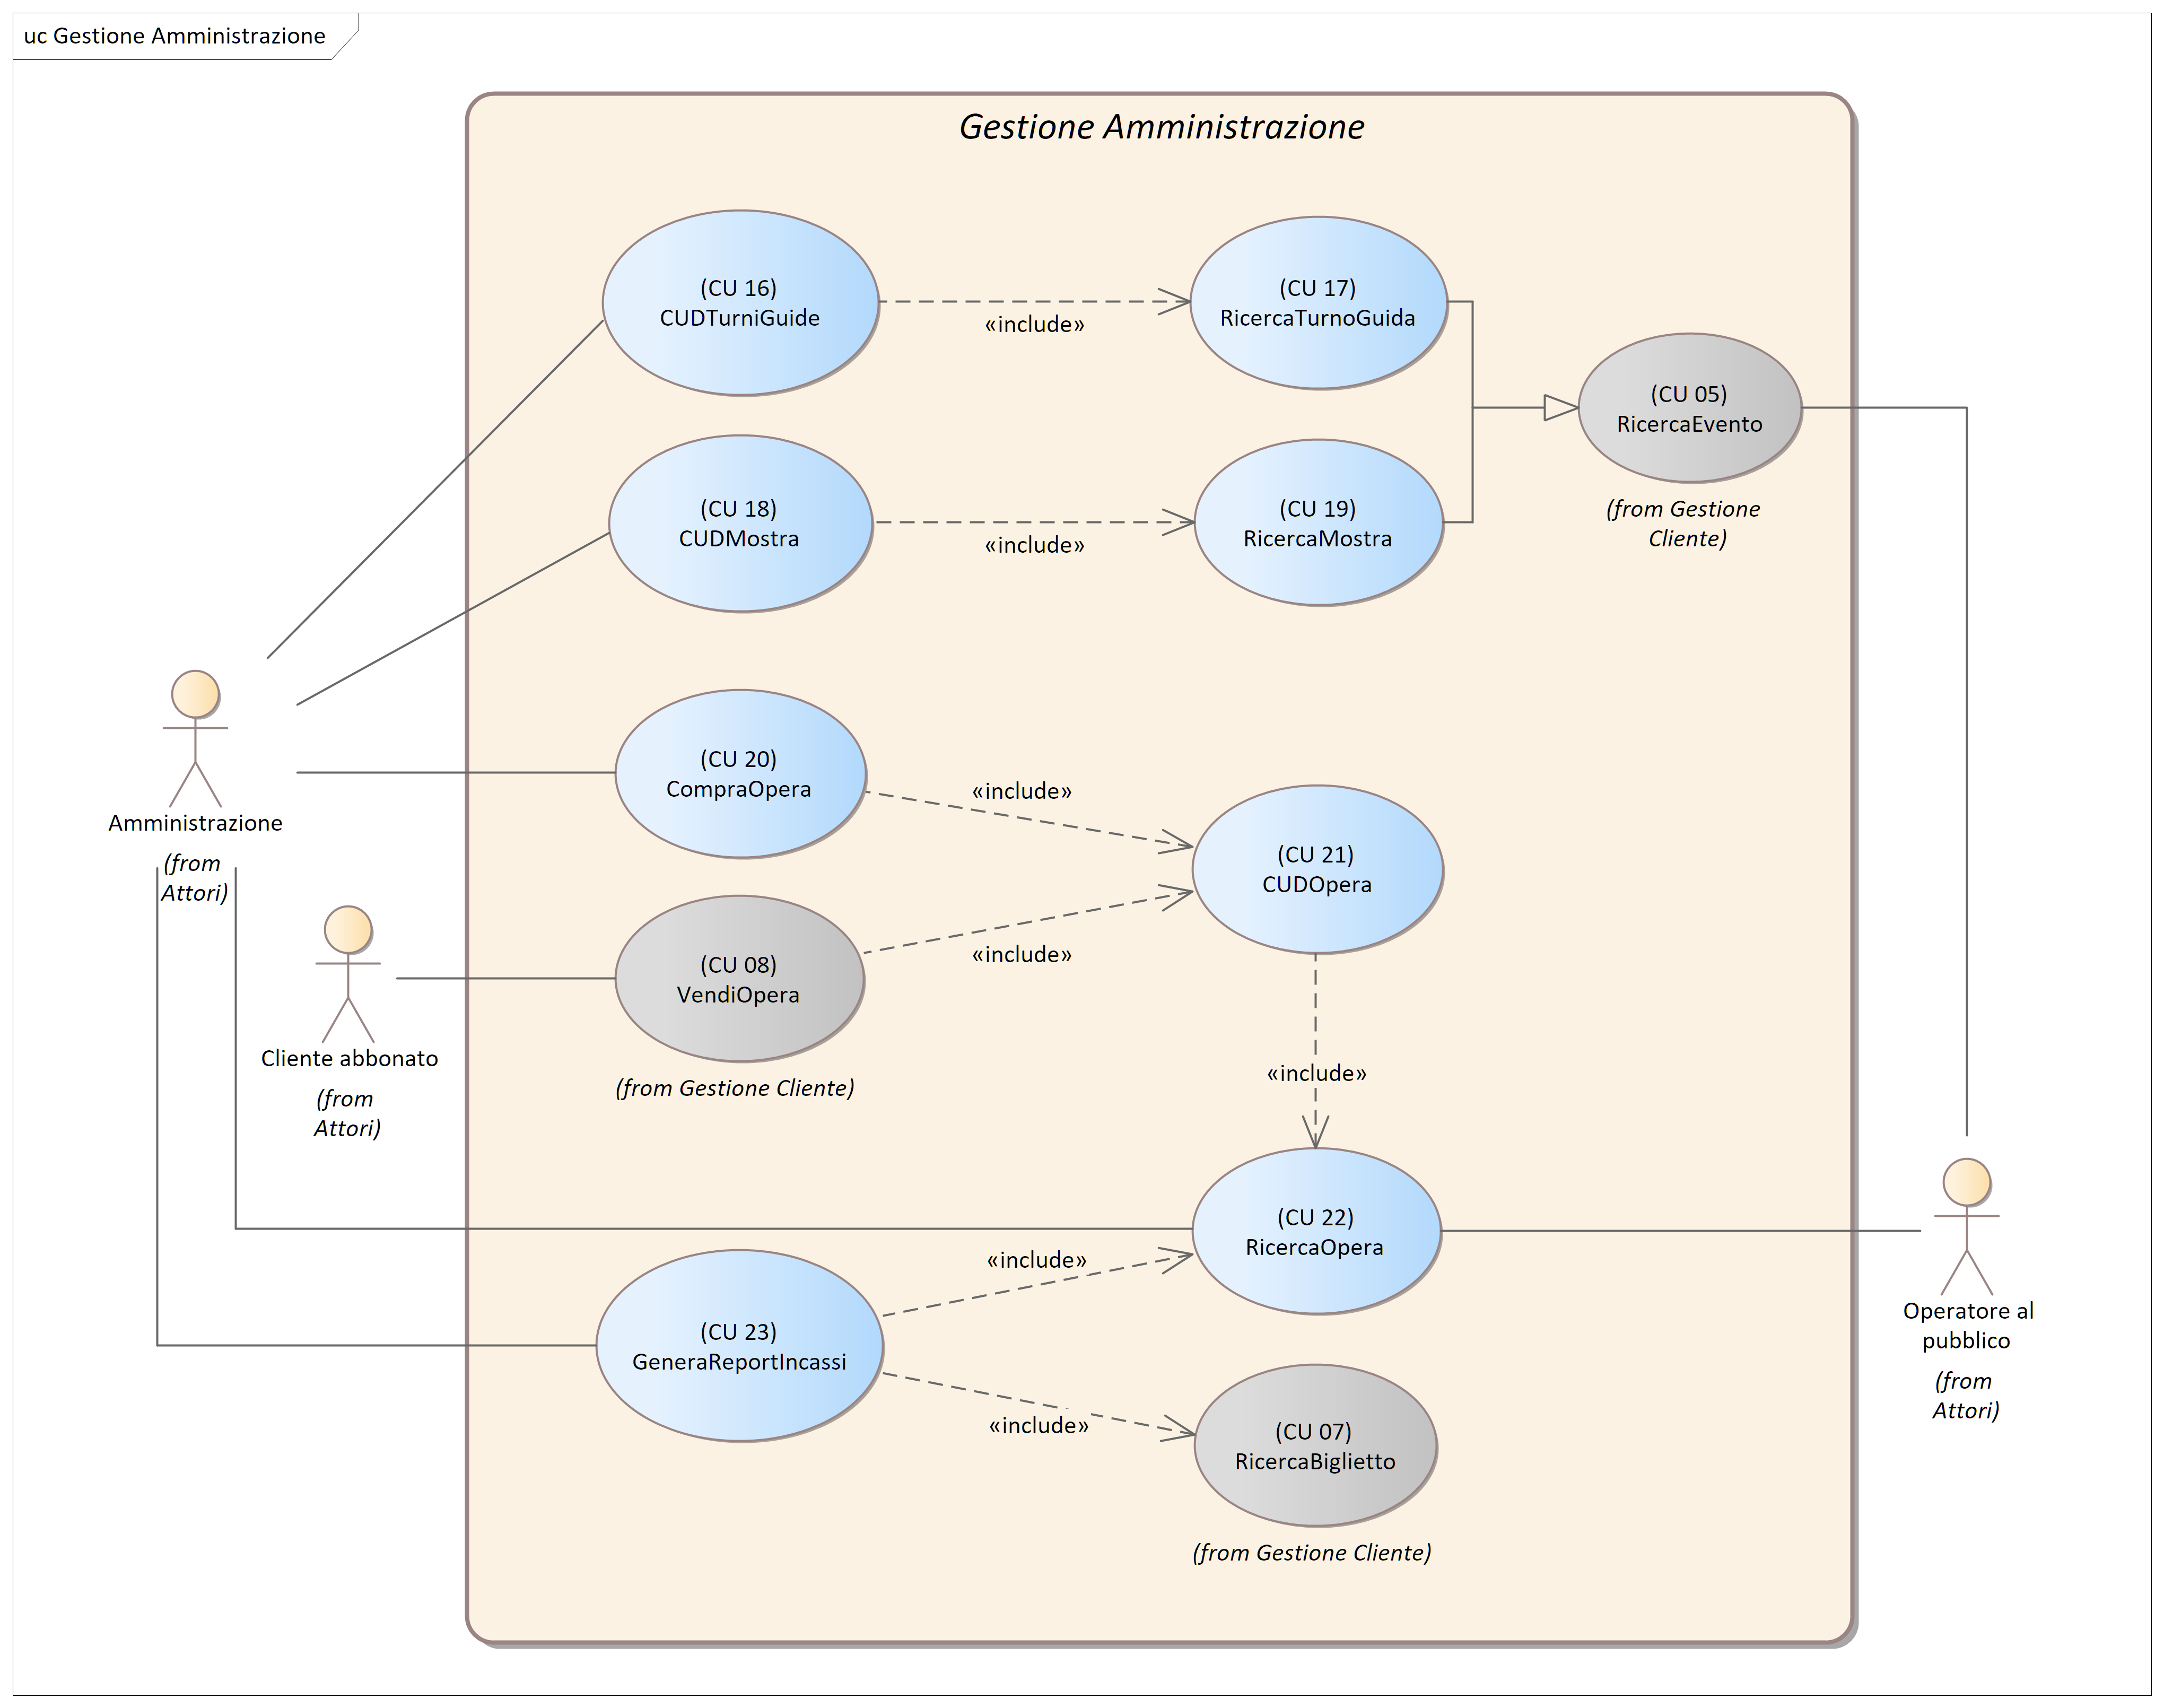
\includegraphics[width=1\textwidth]{Gestione Amministrazione}
    \caption{diagramma dei casi d'uso: \textbf{Gestione Amministrazione}}
    \label{fig:GestioneAmministrazione}
\end{figure}

\newpage

\section*{CUDTurniGuide (CU 16)}
	
\indent\indent Questo caso d'uso consente l’inserimento, la modifica e la rimozione dei turni relativi alle guide che effettueranno i tour della mostra.
	
	\paragraph{Attori primari:}Anmministrazione.
	
	\paragraph{Attori secondari:}Nessuno.
	
	\paragraph{Precondizioni:}
		\begin{enumerate}	[itemsep=8pt,parsep=0pt]
			\item Il sistema ha autenticato l'attore primario.
		\end{enumerate}
	
	\paragraph{Postcondizioni:}
\begin{enumerate}	[itemsep=8pt,parsep=0pt]
\item Il sistema ha memorizzato tutte le modifiche nel database dei turni guide.
\end{enumerate}
	
	\paragraph{Sequenza eventi principale:}

		\begin{enumerate}[itemsep=8pt,parsep=0pt]
		
		\item 
		Il caso d'uso inizia quando l'attore primario vuole effettuare un’operazione CUD relativa ai turni delle guide.


		\item \texttt{\textbf{if}} l'attore primario vuole inserire un nuovo turno:
			\begin{enumerate}	[leftmargin=28pt]
			    \item L'attore inserisce l'ora del nuovo turno e il nome dell' operatore al pubblico.
				\item \texttt{{include(RicercaTurnoGuida)}}
				\item  Il sistema provvede ad aggiungere il nuovo turno.
  			\end{enumerate}	


		\item \texttt{\textbf{else if}} l’attore primario vuole modificare un turno già esistente:
			\begin{enumerate}[leftmargin=28pt]
			    \item L'attore primario inserisce l'ora del turno da modificare e il nome dell' operatore al pubblico.
				\item  \texttt{{include(RicercaTurnoGuida)}}
				\item L'attore primario inserisce l'ora dove spostare il turno.
				\item  \texttt{{include(RicercaTurnoGuida)}}
				\item  Il sistema provvede a modificare l'orario del turno.
  			\end{enumerate}	
  			
  		\item \texttt{\textbf{else if}} l'attore primario vuole eliminare un turno:
			\begin{enumerate}	[leftmargin=28pt]
			\item L'attore primario inserisce l'ora del turno da eliminare e il nome dell' operatore al pubblico.
			\item \texttt{{include(RicercaTurnoGuida)}}
			\item  Il sistema mostra un messaggio di conferma.
			\item \texttt{\textbf{if}}  l'attore primario conferma l'operazione:
			\begin{enumerate}	[leftmargin=28pt]
				\item  Il sistema provvede ad eliminare il turno.
			\end{enumerate}
  		\end{enumerate}		
  			

	\end{enumerate}
	
	\paragraph{Sequenza eventi alternativa: \textit{TurnoGiàEsistente}}
	\begin{enumerate}	[leftmargin=28pt]
			\item  La sequenza di eventi alternativa inizia dopo il passo 2.2. \textbf{or} 3.4. della sequenza di eventi principale.
			\item  Il sistema mostra un opportuno messaggio di errore informando che per l'operatore al pubblico indicato è già programmato un turno nell'orario scelto.
		\end{enumerate}
		
	\paragraph{Sequenza eventi alternativa: \textit{TurnoNonTrovato}}
	\begin{enumerate}	[leftmargin=28pt]
			\item  La sequenza di eventi alternativa inizia dopo il passo 3.2. \textbf{or} 4.2. della sequenza di eventi principale.
			\item  Il sistema mostra un opportuno messaggio di errore informando che non è stato trovato un turno relativo ai parametri di ricerca.
		\end{enumerate}
	
	
	
	
	
	
	
	

	
	
\newpage 

		\section*{RicercaTurnoGuida (CU 17)}
	
	\indent\indent Questo caso d'uso consente di ricercare un turno di una guida. 

	\paragraph{ID padre:}(CU 05).
	
	\paragraph{Attori primari:}Amministrazione, Operatore al pubblico.
	
	\paragraph{Attori secondari:}Nessuno.
	
	\paragraph{Precondizioni:}Nessuna.
	
	\paragraph{Postcondizioni:}Nessuna.
	
	\paragraph{Sequenza eventi principale:}

		\begin{enumerate}[itemsep=8pt,parsep=0pt]

		\item (o 1.) Il caso d'uso inizia quando l'attore primario vuole effettuare la ricerca di un turno di una guida  \texttt{\textbf{or}} il sistema deve effettuare la ricerca di un turno di una guida.

		\item (2.) \texttt{\textbf{if}} il caso d'uso è stato avviato dall'attore:
			\begin{enumerate}	[leftmargin=28pt]
				\item (2.1.) Il sistema chiede i criteri di ricerca.
				\item (o 2.2.) \texttt{\textbf{if}} l'attore non inserisce la data \texttt{\textbf{nor}} il nome della guida:
					\begin{enumerate}	[leftmargin=28pt]
						\item Il sistema usa la data attuale come parametro di ricerca.
		  			\end{enumerate}	
  			\end{enumerate}	

		\item (3.) Il sistema registra i parametri di ricerca.

		\item (o 4.) \texttt{\textbf{for each}} turno nel database dei turni delle guide:
			\begin{enumerate}	[leftmargin=28pt]
				\item (o 4.1.) Il sistema controlla se il turno soddisfa i criteri di ricerca.
				\item (o 4.2.) \texttt{\textbf{if}} il turno soddisfa il criterio:
					\begin{enumerate}	[leftmargin=28pt]
						\item (o 4.2.1.) Il sistema aggiunge il turno alla lista dei risultati.
		  			\end{enumerate}	
  			\end{enumerate}	

		\item (o 5.) \texttt{\textbf{if}} la lista dei risultati contiene almeno un turno:
			\begin{enumerate}	[leftmargin=28pt]
				\item (5.1.) Il sistema mostra la lista dei risultati con tutte le loro informazioni.
  			\end{enumerate}	

		\item (6.) \texttt{\textbf{else}}:
			\begin{enumerate}	[leftmargin=28pt]
				\item (o 6.1.) Il sistema comunica all'attore che nessun turno di alcuna guida soddisfa il criterio specificato.
  			\end{enumerate}	
		
\end{enumerate}	
	
	\paragraph{Sequenza eventi alternativa:}Nessuna. 












	
	
	
	
	
	\newpage 

    \section*{CUDMostra (CU 18)}
	
	\indent\indent Questo caso d'uso consente l’inserimento, la modifica e la rimozione di una mostra.
	
	\paragraph{Attori primari:}Anmministrazione.
	
	\paragraph{Attori secondari:}Nessuno.
	
	\paragraph{Precondizioni:}
		\begin{enumerate}	[itemsep=8pt,parsep=0pt]
			\item Il sistema ha autenticato l'attore primario.
		\end{enumerate}
	
	\paragraph{Postcondizioni:}
\begin{enumerate}	[itemsep=8pt,parsep=0pt]
\item Il sistema ha memorizzato tutte le modifiche nel database delle mostre.
\end{enumerate}
	
	\paragraph{Sequenza eventi principale:}

		\begin{enumerate}[itemsep=8pt,parsep=0pt]
		
		\item 
		Il caso d'uso inizia quando l'attore primario vuole effettuare un’operazione CUD relativa alla mostra.



		\item \texttt{\textbf{if}} l'attore primario vuole inserire una nuova mostra:
			\begin{enumerate}	[leftmargin=28pt]
				\item Il sistema chiede all'attore primario la data nella quale egli desideri organizzare una mostra.
			    \item  \texttt{{include(RicercaMostra)}}
			    %\item  \texttt{{include(RicercaOpera)}}
			    \item \texttt{\textbf{for each}} opera nel database:
			    \begin{enumerate}	[leftmargin=28pt]
					\item Il sistema aggiunge l'opera alla schermata.
			       % \item l'attore primario sceglie se inserire l'opera nella mostra.
                \end{enumerate}
				\item Il sistema chiede all'attore di selezionare le opere da aggiungere alla mostra.
				
			    \item  Il sistema provvede a creare la nuova mostra.
			
  			\end{enumerate}	



		\item \texttt{\textbf{else if}}  l’attore vuole modificare una mostra esistente:
		    \begin{enumerate}[leftmargin=28pt]
				\item Il sistema chiede all'attore primario la data nella quale egli desideri modificare la mostra.
		    \item  \texttt{{include(RicercaMostra)}}
	       % \item  \texttt{{include(RicercaOpera)}}
	       % \item \texttt{\textbf{for each}} opera nel database:
	        %    \begin{enumerate}	[leftmargin=28pt]
		   %     \item l'attore primario sceglie se mantenere le opere nella mostra, aggiungerne di nuove o eliminarle.
            %    \end{enumerate}
			\item \texttt{\textbf{for each}} opera nella mostra \texttt{\textbf{and for each}} opera nel database, ma non nella mostra:
			    \begin{enumerate}	[leftmargin=28pt]
					\item Il sistema aggiunge l'opera alla schermata.
                \end{enumerate}
			\item L'attore rimuove e aggiunge le opere alla mostra.
            \item  Il sistema provvede a salvare le modifiche.
  			\end{enumerate}	
  			
  		\item \texttt{\textbf{else if}} l'attore primario vuole eliminare una mostra esistente:
			    \begin{enumerate}	[leftmargin=28pt]
				\item Il sistema chiede all'attore primario la data nella quale egli desideri rimuovere la mostra.
			    \item  \texttt{{include(RicercaMostra)}}
				\item  Il sistema mostra un messaggio di conferma.
				\item \texttt{\textbf{if}}  l'attore primario conferma l'operazione:
				    \begin{enumerate}	[leftmargin=28pt]
				    \item  Il sistema provvede ad eliminare la mostra.
				    \end{enumerate}
	            \end{enumerate}
	        
	    \end{enumerate}
	
	\paragraph{Sequenza eventi alternativa: \textit{MostraGiàEsistente}}
	\begin{enumerate}	[leftmargin=28pt]
			\item  La sequenza di eventi alternativa inizia dopo il passo 2.2. della sequenza di eventi principale.
			\item  Il sistema mostra un opportuno messaggio di errore informando che è già programmata una mostra nella data specificata.
		\end{enumerate}
		
	\paragraph{Sequenza eventi alternativa: \textit{MostraNonTrovata}}
	\begin{enumerate}	[leftmargin=28pt]
			\item  La sequenza di eventi alternativa inizia dopo il passo 3.2. \textbf{or} 4.2. della sequenza di eventi principale.
			\item  Il sistema mostra un opportuno messaggio di errore informando che non è stata trovata alcuna mostra nella data specificata.
		\end{enumerate}
		
%	\paragraph{Sequenza eventi alternativa: \textit{OperaNonTrovata}}
%	\begin{enumerate}	[leftmargin=28pt]
%			\item  La sequenza di eventi alternativa inizia dopo il passo 3.2. della sequenza di eventi principale.
%			\item  Il sistema mostra un opportuno messaggio di errore informando che non è stata trovata nessun opera relativa ai %parametri di ricerca.
%		\end{enumerate}
	
	
	




	\newpage 

		\section*{RicercaMostra (CU 19)}
	
	\indent\indent Questo caso d'uso consente di ricercare una mostra. 

	\paragraph{ID padre:}(CU 05).
	
	\paragraph{Attori primari:}Amministrazione, Operatore al pubblico.
	
	\paragraph{Attori secondari:}Nessuno.
	
	\paragraph{Precondizioni:}Nessuna.
	
	\paragraph{Postcondizioni:}Nessuna.
	
	\paragraph{Sequenza eventi principale:}

		\begin{enumerate}[itemsep=8pt,parsep=0pt]

		\item (o 1.) Il caso d'uso inizia quando l'attore primario vuole effettuare la ricerca di una mostra  \texttt{\textbf{or}} il sistema deve effettuare la ricerca di una mostra.

		\item (2.) \texttt{\textbf{if}} il caso d'uso è stato avviato dall'attore:
			\begin{enumerate}	[leftmargin=28pt]
				\item (2.1.) Il sistema chiede i criteri di ricerca.
				\item (o 2.2.) \texttt{\textbf{if}} l'attore non inserisce la data \texttt{\textbf{nor}} il nome della mostra:
					\begin{enumerate}	[leftmargin=28pt]
						\item Il sistema usa la data attuale come parametro di ricerca.
		  			\end{enumerate}	
  			\end{enumerate}	

		\item (3.) Il sistema registra i parametri di ricerca.

		\item (o 4.) \texttt{\textbf{for each}} mostra nel database delle mostre:
			\begin{enumerate}	[leftmargin=28pt]
				\item (o 4.1.) Il sistema controlla se la mostra soddisfa i criteri di ricerca.
				\item (o 4.2.) \texttt{\textbf{if}} la mostra soddisfa il criterio:
					\begin{enumerate}	[leftmargin=28pt]
						\item (o 4.2.1.) Il sistema aggiunge la mostra alla lista dei risultati.
		  			\end{enumerate}	
  			\end{enumerate}	

		\item (o 5.) \texttt{\textbf{if}} la lista dei risultati contiene almeno una mostra:
			\begin{enumerate}	[leftmargin=28pt]
				\item (5.1.) Il sistema mostra la lista dei risultati con tutte le loro informazioni.
  			\end{enumerate}	

		\item (6.) \texttt{\textbf{else}}:
			\begin{enumerate}	[leftmargin=28pt]
				\item (o 6.1.) Il sistema comunica all'attore che nessuna mostra soddisfa il criterio specificato.
  			\end{enumerate}	
		
\end{enumerate}	
	
	\paragraph{Sequenza eventi alternativa:}Nessuna. 






	

	
	
	
	
	\newpage 
	
	\section*{CompraOpera (CU 20)}
	
	\indent\indent Questo caso d'uso permette di comprare opere da enti esterni, di gestire le relative transazioni di denaro, e di aggiungerle al database delle opere.
	
	\paragraph{Attori primari:}Anmministrazione.
	
	\paragraph{Attori secondari:}Nessuno.
	
	\paragraph{Precondizioni:}
		\begin{enumerate}	[itemsep=8pt,parsep=0pt]
			\item Il sistema ha autenticato l'attore primario.
		\end{enumerate}
	
	\paragraph{Postcondizioni:}
		\begin{enumerate}[itemsep=8pt,parsep=0pt]
			\item Il sistema ha memorizzato la nuova opera nel database insieme a tutte le sue informazioni.
			\item Il sistema ha memorizzato la transazione effettuata per l'acquisto.
		\end{enumerate}
	
	\paragraph{Sequenza eventi principale:}

		\begin{enumerate}[itemsep=8pt,parsep=0pt]
		
		\item Il caso d’uso inizia quando l’attore primario desidera comprare una nuova opera.

		\item \texttt{\textbf{if}} l'attore primario ha già concluso un affare con un ente esterno privatamente:
			\begin{enumerate}	[leftmargin=28pt]
				\item Il sistema chiede all'attore primario di inserire tutti i dettagli dell'opera acquistata.
				\item Il sistema chiede anche le informazioni sul costo della transazione.
			\end{enumerate}
		\item \texttt{\textbf{else}}
			\begin{enumerate}	[leftmargin=28pt]
		        \item Il sistema si collega al sito web per la compravendita di opere tra enti privati.
					\item \texttt{\textbf{for each}} opera disponibile per l'acquisto:
						\begin{enumerate}	[leftmargin=28pt]
							\item Il sistema preleva tutte le sue informazioni e aggiunge l'opera alla schermata.
						\end{enumerate}
			\item l'attore primario seleziona un'opera alle quale è interessato.
			\end{enumerate}

		    \item  Il sistema mostra un messaggio di conferma.
		    \item \texttt{\textbf{if}}  l'attore primario conferma l'operazione:
		        \begin{enumerate}	[leftmargin=28pt]
		        \item  Il sistema provvede a completare l'acquisto memorizzando la transazione.
		        \item \texttt{{include(CUDOpera)}}
		        \end{enumerate}
\end{enumerate}
	
	\paragraph{Sequenza eventi alternativa:} \textbf{\textit{OperazioneAnnullata}}.
	\begin{enumerate}[itemsep=8pt,parsep=0pt]
	\item La sequenza di eventi alternativa inizia in qualunque momento.
	\item L'attore primario annulla l'operazione di acquisto.
	\end{enumerate}

	\paragraph{Sequenza eventi alternativa:} \textbf{\textit{ConnessioneNonRiuscita}}.
	\begin{enumerate}[itemsep=8pt,parsep=0pt]
				\item La sequenza di eventi alternativa inizia dopo il passo 3.1. della sequenza di eventi principale.
	\item Il sistema comunica all'attore primario, in un opportuno messaggio, l'indisponibilità del sito web per la compravendita di opere e lo esorta ad attendere prima di ripetere l'operazione.
	\end{enumerate}




	
	
	
	
	\newpage 
	
	 \section*{CUDOpera (CU 21)}
	
	\indent\indent Questo caso d'uso consente l’inserimento, la modifica e la rimozione di un'opera.
	
	\paragraph{Attori primari:}Anmministrazione.
	
	\paragraph{Attori secondari:}Nessuno.
	
	\paragraph{Precondizioni:}
		\begin{enumerate}	[itemsep=8pt,parsep=0pt]
			\item Il sistema ha autenticato l'attore primario.
		\end{enumerate}
	
	\paragraph{Postcondizioni:}
		\begin{enumerate}	[itemsep=8pt,parsep=0pt]
			\item Il sistema ha memorizzato tutte le modifiche nel database delle opere.
		\end{enumerate}
	
	\paragraph{Sequenza eventi principale:}

		\begin{enumerate}[itemsep=8pt,parsep=0pt]
		
		\item 
		Il caso d'uso inizia quando l'attore primario vuole effettuare un’operazione CUD relativa ad un'opera.



		\item \texttt{\textbf{if}} l'attore primario vuole inserire una nuova opera:
			\begin{enumerate}	[leftmargin=28pt]
			\item L'attore primario inserisce i dati relativi all'opera.
			\item \texttt{{include(RicercaOpera)}}
			\item  Il sistema provvede ad aggiungere la nuova opera.
  			\end{enumerate}	



		\item \texttt{\textbf{else if}}  l’attore vuole modificare un'opera già esistente:
			\begin{enumerate}[leftmargin=28pt]
			    \item L'attore primario inserisce i dati dell'opera da ricercare.
				\item  \texttt{{include(RicercaOpera)}}
		        \item L'attore aggiorna i dati dell'opera.
		        \item  Il sistema provvede a salvare le modifiche.
  			\end{enumerate}	
  			
  		\item \texttt{\textbf{else if}} l'attore primario vuole eliminare un'opera:
			\begin{enumerate}	[leftmargin=28pt]
			\item L'attore primario inserisce i dati dell'opera da eliminare.
				\item \texttt{{include(RicercaOpera)}}
				\item  Il sistema mostra un messaggio di conferma.
				\item \texttt{\textbf{if}}  l'attore primario conferma l'operazione:
				    \begin{enumerate}	[leftmargin=28pt]
				    	   \item  Il sistema provvede ad eliminare l'opera.
				    \end{enumerate}
  			\end{enumerate}		
  			

	\end{enumerate}
	
	
	\paragraph{Sequenza eventi alternativa: \textit{OperaGiàEsistente}}
	\begin{enumerate}	[leftmargin=28pt]
			\item  La sequenza di eventi alternativa inizia dopo il passo 2.2. della sequenza di eventi principale.
			\item  Il sistema mostra un opportuno messaggio di errore informando che l'opera è già presente nel database.
		\end{enumerate}
		
	\paragraph{Sequenza eventi alternativa: \textit{OperaNonTrovata}}
	\begin{enumerate}	[leftmargin=28pt]
			\item  La sequenza di eventi alternativa inizia dopo il passo 3.2. \textbf{or} 4.2. della sequenza di eventi principale.
			\item  Il sistema mostra un opportuno messaggio di errore informando l'attore primario che non è stata trovata alcuna opera conforme ai parametri di ricerca inseriti.
		\end{enumerate}
	
	
	
	
	
	
	
	
	
	
	
	\newpage 
	
	\section*{RicercaOpera (CU 22)}
	
	\indent\indent Questo caso d'uso permette di ricercare opere all'interno del database delle opere.
	
	\paragraph{Attori primari:}Amministrazione, Operatore al pubblico.
	
	\paragraph{Attori secondari:}Nessuno.
	
	\paragraph{Precondizioni:}Nessuna.
	
	\paragraph{Postcondizioni:}Nessuna.
	
	\paragraph{Sequenza eventi principale:}

		\begin{enumerate}[itemsep=8pt,parsep=0pt]
		
		\item Il caso d’uso inizia quando uno degli attori primari vuole effettuare la ricerca di un'opera \texttt{\textbf{or}} il sistema deve ricercare un'opera.

		\item \texttt{\textbf{if}} il caso d'uso è stato avviato da uno degli attori primari:
			\begin{enumerate}	[leftmargin=28pt]
				\item Il sistema chiede i criteri di ricerca.
				\item L'attore inserisce i criteri di ricerca richiesti.
  			\end{enumerate}	

		\item Il sistema preleva i parametri di ricerca.
		
		\item \texttt{\textbf{for each}} opera nel database:
		\begin{enumerate}	[leftmargin=28pt]
		    \item Il sistema confronta i parametri di ricerca con i parametri dell'opera.
            \item \texttt{\textbf{if}} l'opera rispetta i parametri richiesti:
			 \begin{enumerate}	[leftmargin=28pt]
				\item Il sistema aggiunge l'opera alla lista del risultato di ricerca.
			\end{enumerate}
		\end{enumerate}
		\item \texttt{\textbf{if}} il sistema ha trovato almeno un'opera corrispondente ai parametri di ricerca:
		\begin{enumerate}	[leftmargin=28pt]
			\item  Il sistema fornisce tutti i dati relativi alle opere trovate.
		\end{enumerate}
		\item \texttt{\textbf{else}}
		\begin{enumerate}	[leftmargin=28pt]
				\item  Il sistema informa di non aver trovato nessuna opera corrispondente ai parametri ricercati.
		\end{enumerate}
	\end{enumerate}
	
	\paragraph{Sequenza eventi alternativa:} Nessuna.

	
	
	
	
	
	
	
	
	
\newpage 
	
	\section*{GeneraReportIncassi (CU 23)}
	
	\indent\indent Questo caso d'uso consente di generare il report degli incassi su tutte le transazioni effettuate da inizio mese fino al momento della richiesta oppure in mesi precedenti.
	
	\paragraph{Attori primari:}Anmministrazione.%, Tempo.
	
	\paragraph{Attori secondari:}Nessuno.
	
	\paragraph{Precondizioni:}
		\begin{enumerate}	[itemsep=8pt,parsep=0pt]
			\item Il sistema ha autenticato l'attore primario.
		\end{enumerate}
	
	\paragraph{Postcondizioni:}Nessuna.
	
	\paragraph{Sequenza eventi principale:}

		\begin{enumerate}[itemsep=8pt,parsep=0pt]
		
		\item Il caso d’uso inizia quando l’attore primario desidera generare il report degli incassi.
		\item Il sistema chiede all'attore primario il mese nel quale desidera generare il report degli incassi.
		\item \texttt{\textbf{if}} l'attore primario inserisce un mese antecedente il mese corrente:
			\begin{enumerate}	[leftmargin=28pt]
				\item Il sistema utilizza il mese inserito come criterio di ricerca delle transazioni.
  			\end{enumerate}	
		\item \texttt{\textbf{else if}} l'attore primario non inserisce alcuna data:
			\begin{enumerate}	[leftmargin=28pt]
				\item Il sistema utilizza il mese corrente come criterio di ricerca delle transazioni.
  			\end{enumerate}

		\item \texttt{\textbf{for each}} biglietto nel database dei biglietti:
		    \begin{enumerate}	[leftmargin=28pt]
				\item \texttt{{include(RicercaBiglietto)}}
				\item \texttt{\textbf{if}} il biglietto è stato venduto nel mese selezionato:
					\begin{enumerate}	[leftmargin=28pt]
						\item Il sistema aggiunge la transazione alla lista delle transizioni.
		  			\end{enumerate}	
  		    \end{enumerate}

		\item \texttt{\textbf{for each}} abbonamento nel database degli abbonamenti:
		    \begin{enumerate}	[leftmargin=28pt]
				\item \texttt{{include(RicercaAbbonamento)}}
				\item \texttt{\textbf{if}} l'abbonamento è stato venduto \texttt{\textbf{or}} è stato rinnovato nel mese selezionato :
					\begin{enumerate}	[leftmargin=28pt]
						\item Il sistema aggiunge la transazione alla lista delle transizioni.
		  			\end{enumerate}	
  		    \end{enumerate}

		\item \texttt{\textbf{for each}} opera nel database delle opere:
		    \begin{enumerate}	[leftmargin=28pt]
				\item \texttt{{include(RicercaOpera)}}
				\item \texttt{\textbf{if}} l'opera è stata venduta \texttt{\textbf{or}} l'opera è stata acquistata nel mese selezionato :
					\begin{enumerate}	[leftmargin=28pt]
						\item Il sistema aggiunge la transazione alla lista delle transizioni.
		  			\end{enumerate}	
  		    \end{enumerate}

		\item Il sistema emette il report con tutte le transazioni recuperate e calcola il totale degli incassi come differenza tra le entrate e le uscite.

	\end{enumerate}
	
		\paragraph{Sequenza eventi alternativa: \textit{ReportVuoto}}
	\begin{enumerate}	[leftmargin=28pt]
			\item  La sequenza di eventi alternativa inizia dopo il passo 8. della sequenza di eventi principale.
			\item  Il sistema mostra un opportuno messaggio di errore informando l'attore primario dell'assenza di transazione nel mese selezionato.
		\end{enumerate}













\newpage 
	
	\section*{GestisciDipendenti (CU 36)}
	
	\indent\indent Questo caso d'uso consente di gestire i dipendenti che lavorano all'interno del museo.
	
	\paragraph{Attori primari:}Anmministrazione.
	
	\paragraph{Attori secondari:}Nessuno.
	
	\paragraph{Precondizioni:}
		\begin{enumerate}	[itemsep=8pt,parsep=0pt]
			\item Il sistema ha autenticato l'attore primario.
		\end{enumerate}
	
	\paragraph{Postcondizioni:}
		\begin{enumerate}	[itemsep=8pt,parsep=0pt]
			\item Il sistema ha modificato tutte le modifiche effettuate.
		\end{enumerate}
	
	\paragraph{Sequenza eventi principale:}

		\begin{enumerate}[itemsep=8pt,parsep=0pt]
		
		\item Il caso d’uso inizia quando l’attore primario desidera gestire i dipendenti del museo.
		\item Il sistema chiede all'attore primario il reparto da gestire.
		\item \texttt{\textbf{if}} l'attore primario vuole gestire la reception:
			\begin{enumerate}	[leftmargin=28pt]
				\item Il sistema mostra all'attore primario una lista degli operatori al pubblico dipendenti del museo.
				\item L'attore apporta le modifiche necessarie al personale degli operatori al pubblico.
  			\end{enumerate}	
		\item \texttt{\textbf{else if}} l'attore primario vuole gestire la segreteria:
			\begin{enumerate}	[leftmargin=28pt]
				\item Il sistema mostra all'attore primario una lista dei segretari dipendenti del museo.
				\item L'attore apporta le modifiche necessarie al personale dei segretari.
  			\end{enumerate}

		\item \texttt{\textbf{else if}} l'attore primario vuole gestire l'ammistrazione:
			\begin{enumerate}	[leftmargin=28pt]
				\item Il sistema mostra all'attore primario una lista degli amministratori dipendenti del museo.
				\item L'attore apporta le modifiche necessarie al personale degli amministratori.
  			\end{enumerate}

		\item Il sistema memorizza tutte le modifiche effettuate al personale.

	\end{enumerate}
	
	
	
	
	








	
	


















































































	
	
	
	\newpage 

\section{Gestione Sistema}

\indent\indent Il diagramma dei casi d'uso \textbf{Gestione Sistema} racchiude i casi d'uso istanziabili direttamente solo dal sistema stesso, che permettono di eseguire azioni di \texttt{scheduling}, quali effettuare backup locale e su cloud e avvisare i possessori di abbonamenti prossimi alla scadenza. Nel dettaglio, i casi d'uso di pertinenza sono:
\medskip
\begin{itemize}[itemsep=4pt]
  \item \texttt{ControllaAbbonamenti} (CU 24)
  \item \texttt{InviaAvviso} (CU 25)
  \item \texttt{VerificaAbbonamento} (CU 26)
  \item \texttt{EffettuaBackup} (CU 27)
\end{itemize}
\medskip
Gli attori coinvolti in questi casi d'uso sono l'attore \emph{Tempo}, capace di eseguire lo \texttt{scheduling} delle azioni e l'attore \emph{Amministrazione} che ha la facoltà di eseguire un backup anche fuori dall'orario prestabilito dallo scheduler.

\begin{figure}[h]
    \centering
    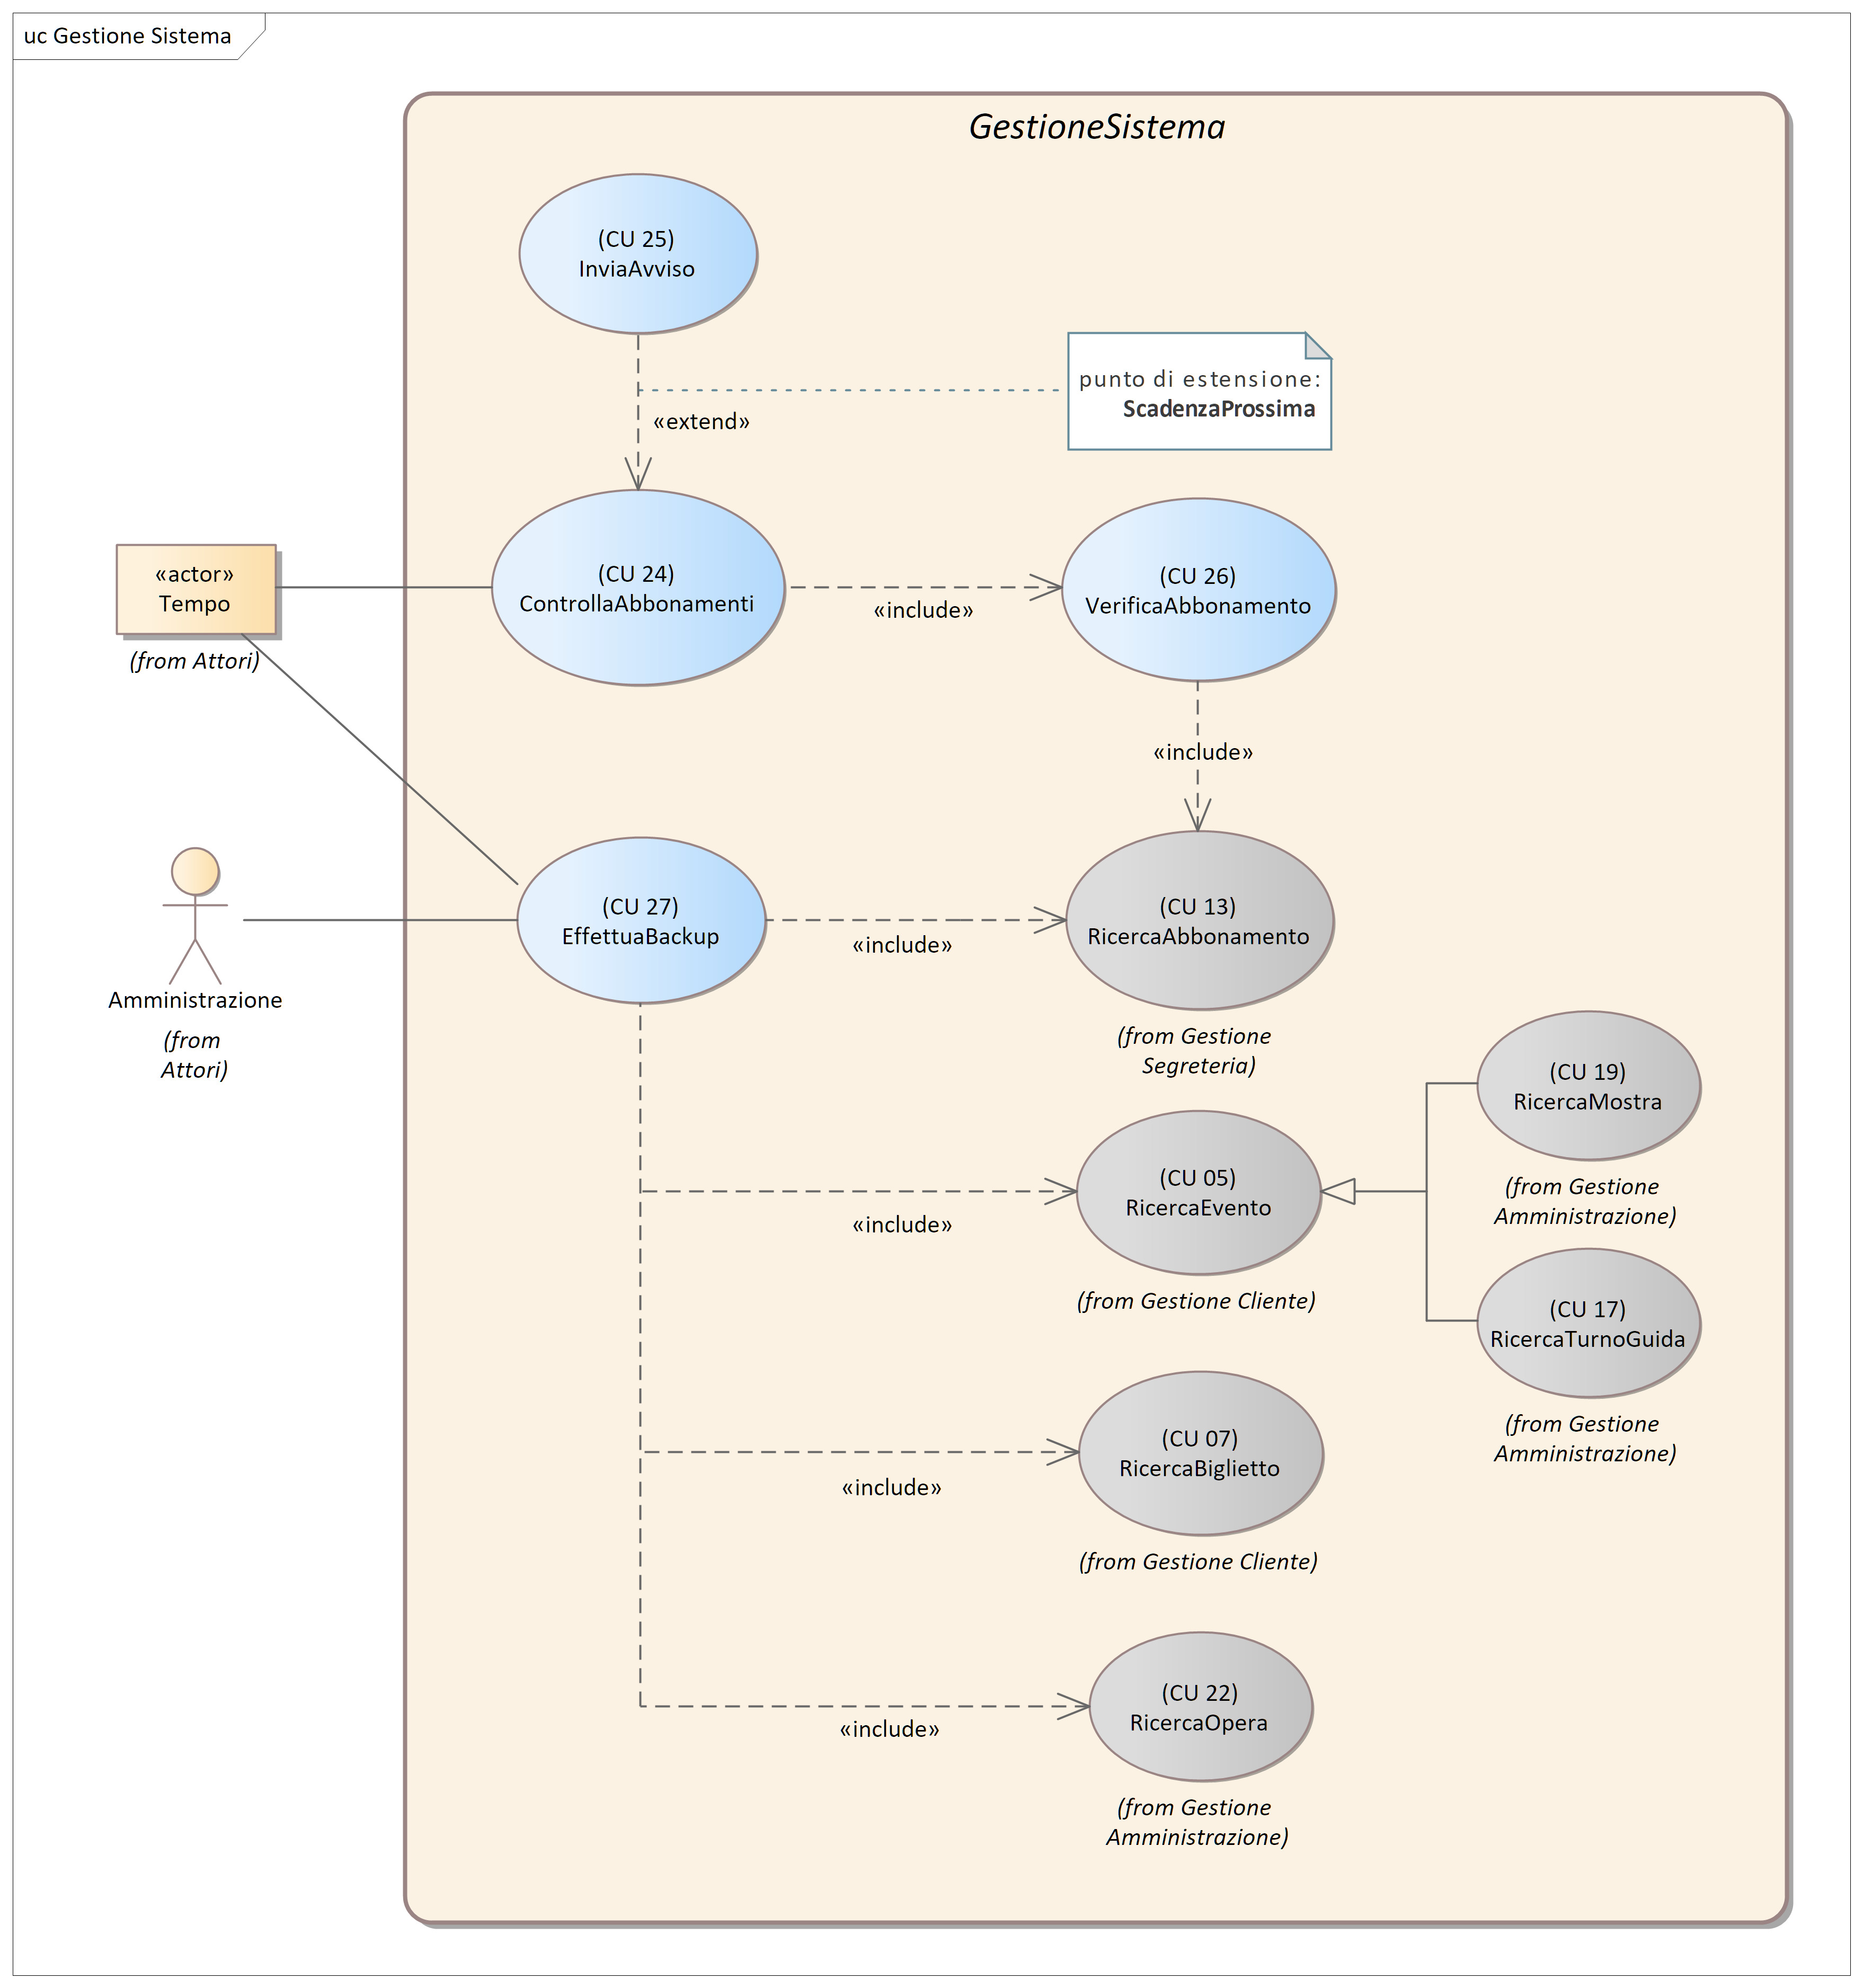
\includegraphics[width=1\textwidth]{Gestione Sistema}
    \caption{diagramma dei casi d'uso: \textbf{Gestione Sistema}}
    \label{fig:GestioneSistema}
\end{figure}

\newpage
	
	
	
	
	
	
	
	
	
	
	
	
	
	
	
\section*{ContollaAbbonamenti (CU 24)}
    
  \indent\indent   Questo caso d'uso consente di controllare gli abbonamenti attivi e segnalare con un avviso i possessori di abbonamenti con scadenza imminente.
    
    \paragraph{Attori primari:}Tempo.
	
	\paragraph{Attori secondari:}Nessuno.
	
	\paragraph{Precondizioni:}Nessuna.
	
	\paragraph{Postcondizioni:}
        \begin{enumerate}	[leftmargin=28pt]
		\item Gli abbonamenti sono stati controllati.
        \end{enumerate}
	
	\paragraph{Sequenza eventi principale:}
\begin{enumerate}[itemsep=8pt,parsep=0pt]
    
    \item
    Il caso d’uso inizia ogni giorno alle ore 23:59 secondo il fuso orario locale.
    
    \item\texttt{\textbf{for each}} abbonanemento nel database degli abbonamenti:
        \begin{enumerate}	[leftmargin=28pt]
			    \item   \texttt{include(VerificaAbbonamento)}
			    \item \texttt{extention point: scadenzaProssima}
			\item Il sistema aggiorna la data di ultimo controllo dell'abbonamento con la data attuale.
                
			    
         \end{enumerate}
	\end{enumerate}
    
	\paragraph{Sequenza eventi alternativa:} Nessuna.
    	
	



	\section*{}
\par\noindent\rule{\textwidth}{0.4pt}
	
\section*{InviaAvviso (CU 25)}
	
\indent\indent Segmento 1: Questo caso d'uso permette al sistema di inviare un avviso ai clienti possessori di un abbonamento in fase di scadenza.
	
	\paragraph{Attori primari:}Tempo.
	
	\paragraph{Attori secondari:}Nessuno.
	
	\paragraph{Precondizioni del segmento 1:}
		\begin{enumerate}	[leftmargin=28pt]
			\item La data di scadenza dell’abbonamento antecede la data corrente di meno di 5 giorni.
	    	\end{enumerate}
	\paragraph{Postcondizioni del segmento 1:} 
		\begin{enumerate}	[leftmargin=28pt]
			\item Il sistema ha inviato una comunicazione via posta elettronica al possessore dell'abbonamento.
	    	\end{enumerate}

	\paragraph{Sequenza eventi principale del segmento 1:}
		\begin{enumerate}[itemsep=8pt,parsep=0pt]
			\item Il caso d'uso inizia quando il sistema deve mandare un messaggio di avviso per rinnovare un abbonamento.
		        \item Il sistema preleva l'indirizzo di posta elettronica dall'abbonamento.
			\item Il sistema genera un messaggio di avviso di rinnovo dell'abbonamento personalizzato e lo invia all'indirizzo di posta elettronica prelevato.
             \end{enumerate}  		
	
	\paragraph{Sequenza eventi alternativa del segmento 1:} Nessuna.	
	
	
	
	
	
	
	
	
	\newpage

\section*{VerificaAbbonamento (CU 26)}
    
   \indent\indent  Questo caso d'uso permette di controllare se un abbonamento è valido, scaduto o in fase di scadenza.
    
    \paragraph{Attori primari:}Segreteria, Operatore al Pubblico, 	Tempo.
	
	\paragraph{Attori secondari:}Nessuno.
	
	\paragraph{Precondizioni:}
\begin{enumerate}[itemsep=8pt,parsep=0pt]
\item Il sistema ha ricevuto l'identificativo dell'abbonamento da controllare.
\end{enumerate}	
	\paragraph{Postcondizioni:}
\begin{enumerate}[itemsep=8pt,parsep=0pt]
\item Il sistema ha verificato lo stato dell'abbonamento.
\end{enumerate}	
	
	\paragraph{Sequenza eventi principale:}
\begin{enumerate}[itemsep=8pt,parsep=0pt]
    
    \item Il caso d’uso inizia quando l'attore primario vuole verificare lo stato di un abbonamento \texttt{\textbf{or}} il sistema deve verificare lo stato di un abbonamento.
    
    \item \texttt{include(RicercaAbbonamento)}

	\item Il sistema legge la data di scadenza dell'abbonamento e la confronta con la data corrente.
    
    \item \texttt{\textbf{if}} la data di scadenza dell’abbonamento precede la data corrente:
          \begin{enumerate}	[leftmargin=28pt]
          \item Il sistema informa l'attore primario che l'abbonamento è scaduto.
          \end{enumerate}

          \item\texttt{\textbf{else if}}  la data di scadenza dell’abbonamento antecede la data corrente di meno di 5 giorni:
	          \begin{enumerate}	[leftmargin=28pt]
	          	\item Il sistema informa l'attore primario che l'abbonamento è in fase di scadenza.
	          \end{enumerate}
\end{enumerate}
    
	\paragraph{Sequenza eventi alternativa:} \textbf{\textit{AbbonamentoNonTrovato}}.
	\begin{enumerate}[itemsep=8pt,parsep=0pt]
		\item La sequenza di eventi alternativa inizia dopo il passo 2. della sequenza di eventi principale.
		\item Il sistema mostra un opportuno messaggio di errore comunicando all'attore primario di non aver trovato alcun abbonamento avente lo stesso codice identificativo inserito, e lo esorta a ripetere il processo di scannerizzazzione del codice QR sul fronte dell'abbonamento.
	\end{enumerate}
    
    	\paragraph{Sequenza eventi alternativa:} \textbf{\textit{OperazioneAnnullata}}.
	\begin{enumerate}[itemsep=8pt,parsep=0pt]
	\item La sequenza di eventi alternativa inizia in qualunque momento.
	\item L'attore primario annulla l'operazione verifica dell'abbonamento.
	\end{enumerate}
    
    
    
    


\newpage

\section*{EffettuaBackup (CU 27)}
	
	\indent\indent Questo caso d’uso consente di effettuare il backup dei dati relativi al sistema informativo di riferimento.
	
	\paragraph{Attori primari:}Amministrazione, Tempo.
	
	\paragraph{Attori secondari:}Amministrazione.
	
	\paragraph{Precondizioni:}
		\begin{enumerate}	[itemsep=8pt,parsep=0pt]
			\item Se il caso d'uso è stato avviato dall'attore primario \emph{Amministrazione}, Il sistema lo ha autenticato.
		\end{enumerate}
	
	\paragraph{Postcondizioni:}I dati sono stati copiati.
	
	\paragraph{Sequenza eventi principale:}
\begin{enumerate}[itemsep=8pt,parsep=0pt]
		
		\item Il caso d'uso inizia ogni sera alle 23:59 secondo il fuso orario locale.

		%\item Il sistema preleva i dati del cliente.                      Quali sono questi dati del cliente?
		%\item Il sistema copia sul disco i dati prelevati.

  		\item \texttt{\textbf{for each}} biglietto nel database dei biglietti:
	          \begin{enumerate}	[leftmargin=28pt]
			\item  \texttt{{include(RicercaBiglietto)}}.
	          	\item Il sistema preleva tutte le informazioni riguardati quel biglietto.
			\item Il sistema copia sul disco i dati del biglietto.
	          \end{enumerate}

  		\item \texttt{\textbf{for each}} abbonamento nel database degli abbonamenti:
	          \begin{enumerate}	[leftmargin=28pt]
			\item  \texttt{{include(RicercaAbbonamento)}}.
	          	\item Il sistema preleva tutte le informazioni riguardati quell'abbonamento.
			\item Il sistema copia sul disco i dati dell'abbonamento.
	          \end{enumerate}

  		\item \texttt{\textbf{for each}} opera nel database delle opere:
	          \begin{enumerate}	[leftmargin=28pt]
			\item  \texttt{{include(RicercaOpera)}}.
	          	\item Il sistema preleva tutte le informazioni riguardati quell'opera.
			\item Il sistema copia sul disco i dati dell'opera.
	          \end{enumerate}

  		\item \texttt{\textbf{for each}} evento nel database degli eventi:
	          \begin{enumerate}	[leftmargin=28pt]
			\item  \texttt{{include(RicercaEvento)}}.
	          	\item Il sistema preleva tutte le informazioni riguardati quell'evento.
			\item Il sistema copia sul disco i dati dell'evento.
	          \end{enumerate}

  		\item \texttt{\textbf{for each}} dato sul visitatore nel database dei dati sui visitatori:
	          \begin{enumerate}	[leftmargin=28pt]
	          	\item Il sistema preleva tutte le informazioni riguardati quel visitatore.
			\item Il sistema copia sul disco i dati del visitatore.
	          \end{enumerate}


		\item Il sistema organizza in una cartella adeguata i dati copiati.
		\item Il sistema effettua l'upload sul cloud utilizzato dal museo del backup appena effettuato.
	\end{enumerate}
	
    	\paragraph{Sequenza eventi alternativa:} \textbf{\textit{DiscoPieno}}.
	\begin{enumerate}[itemsep=8pt,parsep=0pt]
	\item La sequenza di eventi alternativa inizia dopo il passo 6. della sequenza di eventi principale.
	\item Il sistema invia un avviso all'attore secondario comunicante l'impossibilita di effettuare il backup sul disco locale per via della mancanza di spazio sufficiente, e lo esorta a risolvere il problema.
	\end{enumerate}

    	\paragraph{Sequenza eventi alternativa:} \textbf{\textit{UploadNonRiuscito}}.
	\begin{enumerate}[itemsep=8pt,parsep=0pt]
	\item La sequenza di eventi alternativa inizia dopo il passo 7. della sequenza di eventi principale.
	\item Il sistema notifica all'attore secondario l'impossibilità di effettuare l'upload del backup sul cloud e visualizza l'errore.
	\end{enumerate}














































































































\newpage 

\section{Gestione Statistiche}

\indent\indent Il diagramma dei casi d'uso \textbf{Gestione Statistiche} racchiude i casi d'uso necessari per la raccolta dei dati sui clienti in forma anonima e la generazione delle statistiche in base all provenienza, all'età e al sesso del visitatore. Nel dettaglio, i casi d'uso di pertinenza sono:
\medskip
\begin{itemize}[itemsep=4pt]
  \item \texttt{InserisciDatiCliente} (CU 28)
  \item \texttt{InserisciProvenienza} (CU 29)
  \item \texttt{InserisciEtà} (CU 30)
  \item \texttt{InserisciSesso} (CU 31)
  \item \texttt{VisualizzaStatistiche} (CU 32)
  \item \texttt{VisualizzaPerProvenienza} (CU 33)
  \item \texttt{VisualizzaPerEtà} (CU 34)
  \item \texttt{VisualizzaPerSesso} (CU 35)
\end{itemize}
\medskip
Gli attori coinvolti in questi casi d'uso sono l' \emph{Operatore al pubblico} per la popolazione dei dati sui quali inferire le statistiche e  l' \emph{Amministrazione} per la visualizzazione delle stesse.

\begin{figure}[h]
    \centering
    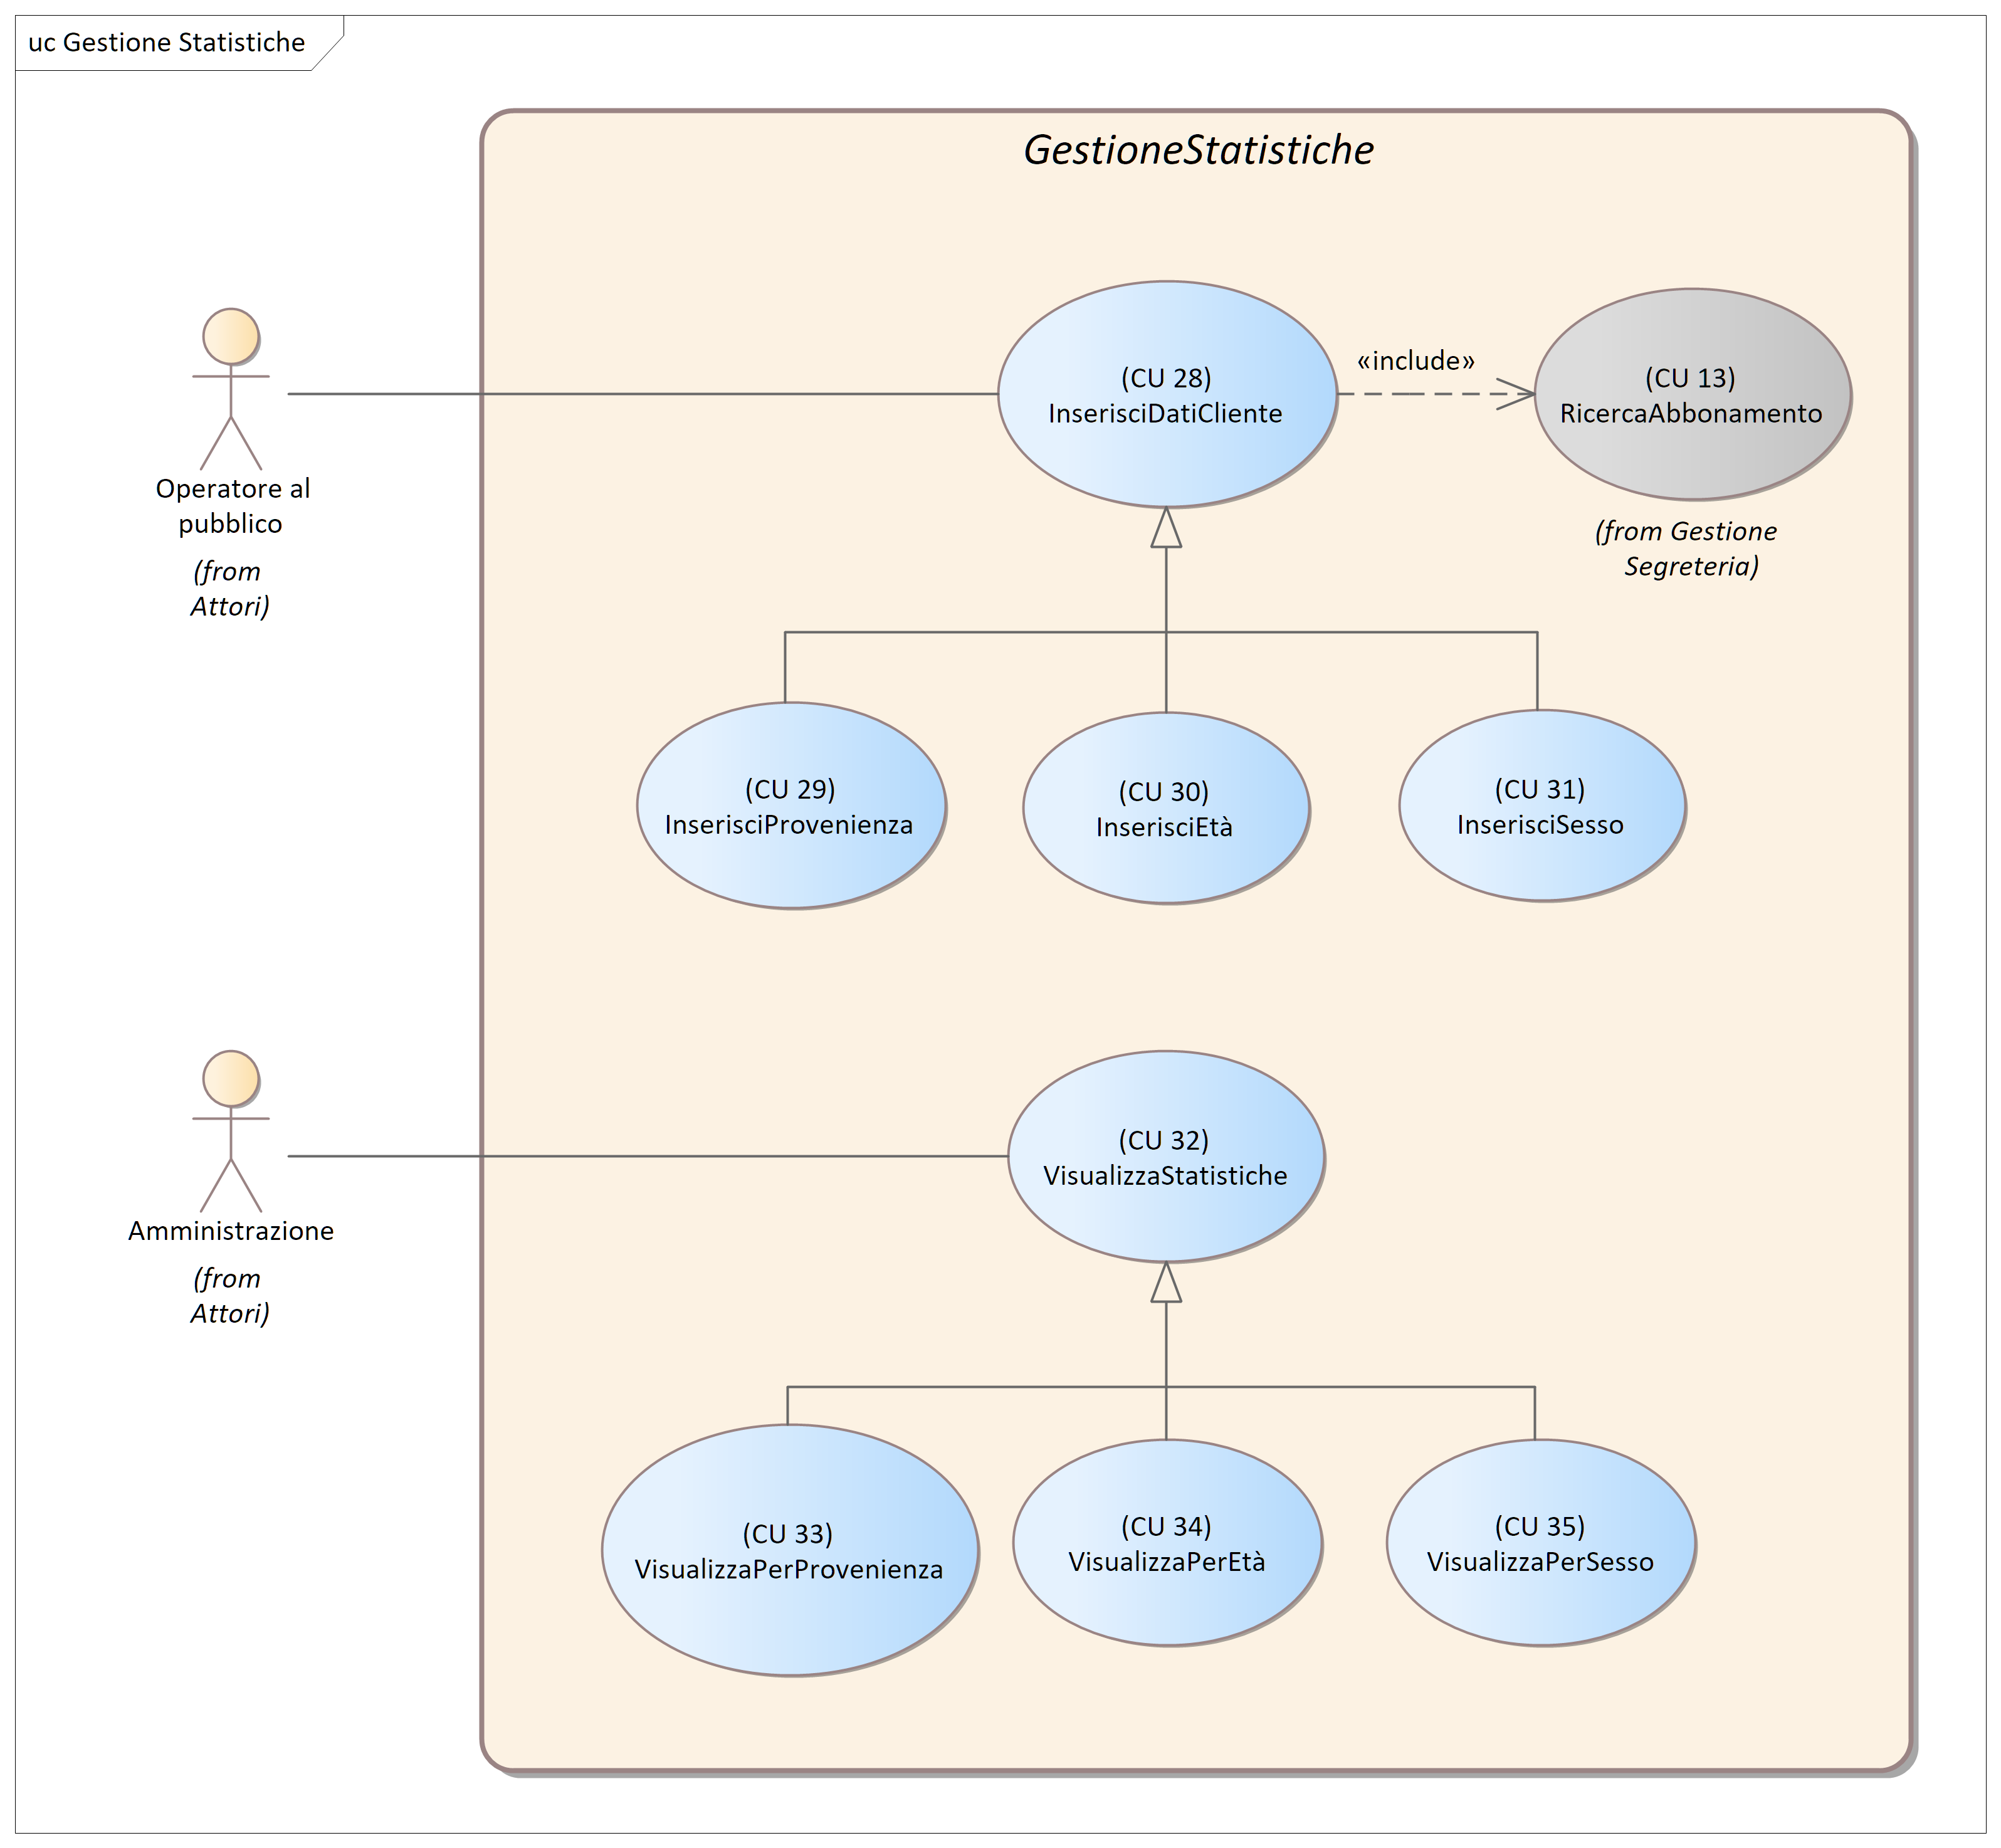
\includegraphics[width=1\textwidth]{Gestione Statistiche}
    \caption{diagramma dei casi d'uso: \textbf{Gestione Statistiche}}
    \label{fig:GestioneStatistiche}
\end{figure}

\newpage

\section*{InserisciDatiCliente (CU 28)}
	
\indent\indent Questo caso d'uso consente di inserire i dati del cliente al momento dell'acquisto del biglietto.
	
	\paragraph{Attori primari:}Operatore al pubblico.
	
	\paragraph{Attori secondari:}Cliente.
	
	\paragraph{Precondizioni:}
	\begin{enumerate}[itemsep=8pt,parsep=0pt]
		\item Il sistema ha autenticato l'attore primario.
		\item Nel caso in cui il cliente disponga di un abbonamento, l'attore primario ha inserito nel sistema l'identificativo dell'abbonamento eseguendo una scannerizzazione del codice QR.
	\end{enumerate}

	\paragraph{Postcondizioni:}
	\begin{enumerate}[itemsep=8pt,parsep=0pt]
		\item Il sistema ha memorizzato i dati inseriti in forma anonima.
	\end{enumerate}
	
	\paragraph{Sequenza eventi principale:}

	\begin{enumerate}[itemsep=8pt,parsep=0pt]
	    \item Il caso d'uso inizia quando l'attore primario vuole memorizzare i dati di un cliente. 
	    \item \texttt{\textbf{if}} il cliente dispone di un abbonamento:
			\begin{enumerate}	[leftmargin=28pt]
			\item Il sistema recupera i dati necessari dal suo abbonamento. %(Che già ha perché ha preso il suo abbonamento giusto?)
			\item \texttt{{include(RicercaAbbonamento)}}
  			\end{enumerate}
  		\item \texttt{\textbf{else}}:
  		\begin{enumerate}	[leftmargin=28pt]
	        \item L'attore primario chiede al cliente i dati necessari.
	        \item L'attore primario inserisce i dati nel sistema.
	    \end{enumerate}
		\item Il sistema memorizza i dati.
		\item Il sistema produce un messaggio con l'esito dell'operazione.
	
	\end{enumerate}
	
	\paragraph{Sequenza eventi alternativa: \emph{DatiNonFornitiDalCliente}}
		\begin{enumerate}[itemsep=8pt,parsep=0pt]
				\item La sequenza di eventi alternativa inizia dopo il passo 3.1. della sequenza di eventi principale.
				\item L'attore secondario si rifiuta di fornire le informazioni.
				\item L'attore primario annulla l'operazione.
				\item Il sistema termina l'operazione senza memorizzare alcun dato riguardante il cliente.
		\end{enumerate}





	
	
\newpage	
\section*{InserisciProvenienza (CU 29)}
	
	\indent\indent Questo caso d'uso consente di inserire lo Stato di nascita del cliente.
	
	\paragraph{Id padre:}(CU 28)
	
	\paragraph{Attori primari:}Operatore al pubblico.
	
	\paragraph{Attori secondari:}Cliente.
	
	\paragraph{Precondizioni:}
	\begin{enumerate}[itemsep=8pt,parsep=0pt]
		\item Il sistema ha autenticato l'attore primario.
		\item Nel caso in cui il cliente disponga di un abbonamento, l'attore primario ha inserito nel sistema l'identificativo dell'abbonamento eseguendo una scannerizzazione del codice QR.
	\end{enumerate}

	\paragraph{Postcondizioni:}
	\begin{enumerate}[itemsep=8pt,parsep=0pt]
		\item Il sistema ha memorizzato i dati inseriti in forma anonima.
	\end{enumerate}
	
	\paragraph{Sequenza eventi principale:}

	\begin{enumerate}[itemsep=8pt,parsep=0pt]
	    \item(o1) Il caso d'uso inizia quando l'attore primario vuole memorizzare il Paese d'origine del cliente. 
	    \item(2.) \texttt{\textbf{if}} il cliente dispone di un abbonamento:
			\begin{enumerate}	[leftmargin=28pt]
			\item (2.1.) Il sistema recupera i dati necessari dal suo abbonamento. %(Che già ha perché ha preso il suo abbonamento giusto?) Si
			\item (2.2.) \texttt{{include(RicercaAbbonamento)}}
  			\end{enumerate}
  		\item(3.) \texttt{\textbf{else}}:
  		\begin{enumerate}	[leftmargin=28pt]
	        \item(o3.1) L'attore primario chiede al cliente il suo Paese d'origine.
	        \item(o3.2.) L'attore primario inserisce il Paese d'origine del cliente nel sistema.
	    \end{enumerate}
		\item(4.) Il sistema memorizza i dati.
		\item(5.) Il sistema produce un messaggio con l'esito dell'operazione.
	
	\end{enumerate}
	
	\paragraph{Sequenza eventi alternativa: \emph{DatiNonFornitiDalCliente}}
		\begin{enumerate}[itemsep=8pt,parsep=0pt]
				\item (1.) La sequenza di eventi alternativa inizia dopo il passo 3.1. della sequenza di eventi principale.
				\item (o2.) L'attore secondario si rifiuta di fornire l'informazione del suo Paese di origine.
				\item (3.) L'attore primario annulla l'operazione.
				\item (4.) Il sistema termina l'operazione senza memorizzare alcun dato riguardante il cliente.
		\end{enumerate}
	



	
\newpage	
\section*{InserisciEtà (CU 30)}
	
	\indent\indent Questo caso d'uso consente di inserire l'età del cliente.
	
	\paragraph{Id padre:} (CU 28)
	
	\paragraph{Attori primari:}Operatore al pubblico.
	
	\paragraph{Attori secondari:}Cliente.
	
	\paragraph{Precondizioni:}
	\begin{enumerate}[itemsep=8pt,parsep=0pt]
		\item Il sistema ha autenticato l'attore primario.
		\item Nel caso in cui il cliente disponga di un abbonamento, l'attore primario ha inserito nel sistema l'identificativo dell'abbonamento eseguendo una scannerizzazione del codice QR.
	\end{enumerate}

	\paragraph{Postcondizioni:}
	\begin{enumerate}[itemsep=8pt,parsep=0pt]
		\item Il sistema ha memorizzato i dati inseriti in forma anonima.
	\end{enumerate}

	\paragraph{Sequenza eventi principale:}

	\begin{enumerate}[itemsep=8pt,parsep=0pt]
	    \item(o1) Il caso d'uso inizia quando l'attore primario vuole memorizzare la data di nascita del cliente. 
	    \item(2.) \texttt{\textbf{if}} il cliente dispone di un abbonamento:
			\begin{enumerate}	[leftmargin=28pt]
			\item (2.1.) Il sistema recupera i dati necessari dal suo abbonamento. %(Che già ha perché ha preso il suo abbonamento giusto?) Si 
			\item (2.2.) \texttt{{include(RicercaAbbonamento)}}
  			\end{enumerate}
  		\item(3.) \texttt{\textbf{else}}:
  		\begin{enumerate}	[leftmargin=28pt]
	        \item(o3.1) L'attore primario chiede al cliente la sua data di nascita.
	        \item(o3.2.) L'attore primario inserisce la data di nascita del cliente nel sistema.
	    \end{enumerate}
		\item(4.) Il sistema memorizza i dati.
		\item(5.) Il sistema produce un messaggio con l'esito dell'operazione.
	\end{enumerate}

	\paragraph{Sequenza eventi alternativa: \emph{DatiNonFornitiDalCliente}}
		\begin{enumerate}[itemsep=8pt,parsep=0pt]
				\item (1.) La sequenza di eventi alternativa inizia dopo il passo 3.1. della sequenza di eventi principale.
				\item (o2.) L'attore secondario si rifiuta di fornire l'informazione della sua data di nascita.
				\item (3.) L'attore primario annulla l'operazione.
				\item (4.) Il sistema termina l'operazione senza memorizzare alcun dato riguardante il cliente.
		\end{enumerate}
	



	
\newpage
\section*{InserisciSesso (CU 31)}
	
	\indent\indent Questo caso d'uso consente di inserire il genere del cliente.
	
	\paragraph{Id padre:} (CU 28)
	
	\paragraph{Attori primari:}Operatore al pubblico.
	
	\paragraph{Attori secondari:}Cliente.
	
	\paragraph{Precondizioni:}
	\begin{enumerate}[itemsep=8pt,parsep=0pt]
		\item Il sistema ha autenticato l'attore primario.
		\item Nel caso in cui il cliente disponga di un abbonamento, l'attore primario ha inserito nel sistema l'identificativo dell'abbonamento eseguendo una scannerizzazione del codice QR.
	\end{enumerate}

	\paragraph{Postcondizioni:}
	\begin{enumerate}[itemsep=8pt,parsep=0pt]
		\item Il sistema ha memorizzato i dati inseriti in forma anonima.
	\end{enumerate}
	
	\paragraph{Sequenza eventi principale:}

	\begin{enumerate}[itemsep=8pt,parsep=0pt]
	    \item(o1) Il caso d'uso inizia quando l'attore primario vuole memorizzare il genere del cliente. 
	    \item(2.) \texttt{\textbf{if}} il cliente dispone di un abbonamento:
			\begin{enumerate}	[leftmargin=28pt]
			\item (2.1.) Il sistema recupera i dati necessari dal suo abbonamento. %(Che già ha perché ha preso il suo abbonamento giusto?) Si
			\item (2.2.) \texttt{{include(RicercaAbbonamento)}}
  			\end{enumerate}
  		\item(3.) \texttt{\textbf{else}}:
  		\begin{enumerate}	[leftmargin=28pt]
	        \item(o3.1) L'attore primario chiede al cliente il suo genere. % :D
	        \item(o3.2.) L'attore primario inserisce il genere del cliente nel sistema.
	    \end{enumerate}
		\item(4.) Il sistema memorizza i dati.
		\item(5.) Il sistema produce un messaggio con l'esito dell'operazione.
	\end{enumerate}
	
	\paragraph{Sequenza eventi alternativa: \emph{DatiNonFornitiDalCliente}}
		\begin{enumerate}[itemsep=8pt,parsep=0pt]
				\item (1.) La sequenza di eventi alternativa inizia dopo il passo 3.1. della sequenza di eventi principale.
				\item (o2.) L'attore secondario si rifiuta di fornire l'informazione del suo genere.
				\item (3.) L'attore primario annulla l'operazione.
				\item (4.) Il sistema termina l'operazione senza memorizzare alcun dato riguardante il cliente.
		\end{enumerate}
	
	


\newpage	
\section*{VisualizzaStatistiche (CU 32)}
	
	\indent\indent Questo caso d'uso consente di generare statistiche in un particolare mese sulla base dei dati sui clienti raccolti in forma anonima dal sistema.
	
	\paragraph{Attori primari:}Anmministrazione.
	
	\paragraph{Attori secondari:}Nessuno.
	
	\paragraph{Precondizioni:}
	\begin{enumerate}[itemsep=8pt,parsep=0pt]
		\item Il sistema ha autenticato l'attore primario.
	\end{enumerate}
	
	\paragraph{Postcondizioni:}Nessuna.
	
	\paragraph{Sequenza eventi principale:}
	\begin{enumerate}[itemsep=8pt,parsep=0pt]
	    \item Il caso d'uso inizia quando l'attore primario vuole visualizzare le statistiche. 
		\item Il sistema chiede all'attore primario il mese nel quale desidera generare le statistiche.
		\item \texttt{\textbf{if}} l'attore primario inserisce un mese antecedente il mese corrente:
			\begin{enumerate}	[leftmargin=28pt]
				\item Il sistema utilizza il mese inserito come criterio di ricerca.
  			\end{enumerate}	
		\item \texttt{\textbf{else if}} l'attore primario non inserisce alcuna data:
			\begin{enumerate}	[leftmargin=28pt]
				\item Il sistema utilizza il mese corrente come criterio di ricerca.
  			\end{enumerate}

		\item \texttt{\textbf{for each}} dato sul cliente nel database dei dati sui clienti:
		    \begin{enumerate}	[leftmargin=28pt]
				\item \texttt{\textbf{if}} il dato sul cliente è stato registrato nel sistema nel mese selezionato:
					\begin{enumerate}	[leftmargin=28pt]
						\item Il sistema aggiunge il dato sul cliente alla lista dei dati raccolti.
		  			\end{enumerate}	
  		    \end{enumerate}

	    \item Il sistema organizza i dati sulla base dei quali genera un grafico e lo mostra a schermo.
	    \item Il sistema calcola deviazione standard campionaria sulla base dei dati raccolti e mostra a schermo i risultati.
	    \item Il sistema mostra a schermo anche il numero di visite avvenute dall'inizio del mese, fino al momento della richiesta. %(potrebbe essere inserito anche nel punto precedente)
	\end{enumerate}
	
		\paragraph{Sequenza eventi alternativa: \textit{NessunDato}}
	\begin{enumerate}	[leftmargin=28pt]
			\item  La sequenza di eventi alternativa inizia dopo il passo 6. della sequenza di eventi principale.
			\item  Il sistema mostra un opportuno messaggio di errore informando l'attore primario dell'assenza di dati sui clienti nel mese selezionato.
		\end{enumerate}
	





\newpage
\section*{VisualizzaPerProvenienza (CU 33)}
	
	Questo caso d'uso consente di eseguire la ricerca di un abbonamento all'interno del database.
	
	\paragraph{Id padre:} (CU 32)
	
	\paragraph{Attori primari:}Anmministrazione.
	
	\paragraph{Attori secondari:}Nessuno.
	
	\paragraph{Precondizioni:}
	\begin{enumerate}[itemsep=8pt,parsep=0pt]
		\item Il sistema ha autenticato l'attore primario.
	\end{enumerate}
	
	\paragraph{Postcondizioni:}Nessuna.
	
	\paragraph{Sequenza eventi principale:}
	\begin{enumerate}[itemsep=8pt,parsep=0pt]
	    \item (1.) Il caso d'uso inizia quando l'attore primario vuole visualizzare le statistiche. 
		\item (2.) Il sistema chiede all'attore primario il mese nel quale desidera generare le statistiche.
		\item (3.) \texttt{\textbf{if}} l'attore primario inserisce un mese antecedente il mese corrente:
			\begin{enumerate}	[leftmargin=28pt]
				\item (3.1.) Il sistema utilizza il mese inserito come criterio di ricerca.
  			\end{enumerate}	
		\item (4.) \texttt{\textbf{else if}} l'attore primario non inserisce alcuna data:
			\begin{enumerate}	[leftmargin=28pt]
				\item (4.1.) Il sistema utilizza il mese corrente come criterio di ricerca.
  			\end{enumerate}

		\item (5.) \texttt{\textbf{for each}} dato sul cliente nel database dei dati sui clienti:
		    \begin{enumerate}	[leftmargin=28pt]
				\item (5.1.) \texttt{\textbf{if}} il dato sul cliente è stato registrato nel sistema nel mese selezionato:
					\begin{enumerate}	[leftmargin=28pt]
						\item (o5.1.1.) Il sistema aggiunge il Paese di origine del cliente alla lista dei dati raccolti.
		  			\end{enumerate}	
  		    \end{enumerate}

	    \item (o6.) Il sistema organizza i dati sulla base dei quali genera un grafico a torta e lo mostra a schermo.
	    \item (7.) Il sistema calcola la deviazione standard campionaria sulla base dei dati raccolti e mostra a schermo i risultati.
	    \item (8.) Il sistema mostra a schermo anche il numero di visite avvenute dall'inizio del mese, fino al momento della richiesta. %(potrebbe essere inserito anche nel punto precedente)
	\end{enumerate}
	
		\paragraph{Sequenza eventi alternativa: \textit{NessunDato}}
	\begin{enumerate}	[leftmargin=28pt]
			\item  (1.) La sequenza di eventi alternativa inizia dopo il passo 6. della sequenza di eventi principale.
			\item  (2.) Il sistema mostra un opportuno messaggio di errore informando l'attore primario dell'assenza di dati sui clienti nel mese selezionato.
		\end{enumerate}
	
	




\newpage	
\section*{VisualizzaPerEtà (CU 34)}
	
	Questo caso d'uso consente di eseguire la ricerca di un abbonamento all'interno del database.
	
	\paragraph{Id padre:} (CU 32)
	
	\paragraph{Attori primari:}Anmministrazione.
	    
	\paragraph{Attori secondari:}Nessuno.
	
	\paragraph{Precondizioni:}
	\begin{enumerate}[itemsep=8pt,parsep=0pt]
		\item Il sistema ha autenticato l'attore primario.
	\end{enumerate}
	
	\paragraph{Postcondizioni:}Nessuna.
	
	\paragraph{Sequenza eventi principale:}
	\begin{enumerate}[itemsep=8pt,parsep=0pt]
	    \item (1.) Il caso d'uso inizia quando l'attore primario vuole visualizzare le statistiche. 
		\item (2.) Il sistema chiede all'attore primario il mese nel quale desidera generare le statistiche.
		\item (3.) \texttt{\textbf{if}} l'attore primario inserisce un mese antecedente il mese corrente:
			\begin{enumerate}	[leftmargin=28pt]
				\item (3.1.) Il sistema utilizza il mese inserito come criterio di ricerca.
  			\end{enumerate}	
		\item (4.) \texttt{\textbf{else if}} l'attore primario non inserisce alcuna data:
			\begin{enumerate}	[leftmargin=28pt]
				\item (4.1.) Il sistema utilizza il mese corrente come criterio di ricerca.
  			\end{enumerate}

		\item (5.) \texttt{\textbf{for each}} dato sul cliente nel database dei dati sui clienti:
		    \begin{enumerate}	[leftmargin=28pt]
				\item (5.1.) \texttt{\textbf{if}} il dato sul cliente è stato registrato nel sistema nel mese selezionato:
					\begin{enumerate}	[leftmargin=28pt]
						\item (o5.1.1) Il sistema raccoglie la data di nascita del cliente e la utilizza per calcolare l'età.
						\item (5.1.2.) Il sistema aggiunge l'età del cliente alla lista dei dati raccolti.
		  			\end{enumerate}	
  		    \end{enumerate}

	    \item (o6.) Il sistema organizza i dati sulla base dei quali genera un grafico istogramma e lo mostra a schermo.
	    \item (o7.) Il sistema calcola la media campionaria e la deviazione standard campionaria sulla base dei dati raccolti e mostra a schermo i risultati.
	    \item (8.) Il sistema mostra a schermo anche il numero di visite avvenute dall'inizio del mese, fino al momento della richiesta. %(potrebbe essere inserito anche nel punto precedente)
	\end{enumerate}
	
		\paragraph{Sequenza eventi alternativa: \textit{NessunDato}}
	\begin{enumerate}	[leftmargin=28pt]
			\item  (1.) La sequenza di eventi alternativa inizia dopo il passo 6. della sequenza di eventi principale.
			\item  (2.) Il sistema mostra un opportuno messaggio di errore informando l'attore primario dell'assenza di dati sui clienti nel mese selezionato.
		\end{enumerate}




	
	
\newpage
\section*{VisualizzaPerSesso (CU 35)}
	
	Questo caso d'uso consente di eseguire la ricerca di un abbonamento all'interno del database.
	
	\paragraph{Id padre:} (CU 32)
	
	\paragraph{Attori primari:}Anmministrazione.
	
	\paragraph{Attori secondari:}Nessuno.
	
	\paragraph{Precondizioni:}
	\begin{enumerate}[itemsep=8pt,parsep=0pt]
		\item Il sistema ha autenticato l'attore primario.
	\end{enumerate}
	
	\paragraph{Postcondizioni:}Nessuna.

	\paragraph{Sequenza eventi principale:}
	\begin{enumerate}[itemsep=8pt,parsep=0pt]
	    \item (1.) Il caso d'uso inizia quando l'attore primario vuole visualizzare le statistiche. 
		\item (2.) Il sistema chiede all'attore primario il mese nel quale desidera generare le statistiche.
		\item (3.) \texttt{\textbf{if}} l'attore primario inserisce un mese antecedente il mese corrente:
			\begin{enumerate}	[leftmargin=28pt]
				\item (3.1.) Il sistema utilizza il mese inserito come criterio di ricerca.
  			\end{enumerate}	
		\item (4.) \texttt{\textbf{else if}} l'attore primario non inserisce alcuna data:
			\begin{enumerate}	[leftmargin=28pt]
				\item (4.1.) Il sistema utilizza il mese corrente come criterio di ricerca.
  			\end{enumerate}

		\item (5.) \texttt{\textbf{for each}} dato sul cliente nel database dei dati sui clienti:
		    \begin{enumerate}	[leftmargin=28pt]
				\item (5.1.) \texttt{\textbf{if}} il dato sul cliente è stato registrato nel sistema nel mese selezionato:
					\begin{enumerate}	[leftmargin=28pt]
						\item (o5.1.1.) Il sistema aggiunge il genere del cliente alla lista dei dati raccolti.
		  			\end{enumerate}	
  		    \end{enumerate}

	    \item (o6.) Il sistema organizza i dati sulla base dei quali genera un grafico a torta e lo mostra a schermo.
	    \item (7.) Il sistema calcola la deviazione standard campionaria sulla base dei dati raccolti e mostra a schermo i risultati.
	    \item (8.) Il sistema mostra a schermo anche il numero di visite avvenute dall'inizio del mese, fino al momento della richiesta. %(potrebbe essere inserito anche nel punto precedente)
	\end{enumerate}
	
		\paragraph{Sequenza eventi alternativa: \textit{NessunDato}}
	\begin{enumerate}	[leftmargin=28pt]
			\item  (1.) La sequenza di eventi alternativa inizia dopo il passo 6. della sequenza di eventi principale.
			\item  (2.) Il sistema mostra un opportuno messaggio di errore informando l'attore primario dell'assenza di dati sui clienti nel mese selezionato.
		\end{enumerate}


\end{document}








